\section{Our solution}
    \label{sec:contribution}
    For the implementation of the project, the requirements for the software are defined first. The requirements are still general in this, first section and become more concrete during the development of the design. Following the requirement definitions a detailed solution is compiled step by step. The most important concepts of this software are thereby the software architecture, the data model, the function model, the permission model and the user interface. Thus, the software can be developed according to the defined concepts and evaluated afterwards.

    \subsection*{Requirement specifications}
    The goal to be achieved is to combine project management with CAD data to create a compact and lightweight solution. Customers and companies can evaluate and control the development status on a common basis. For this purpose, the platform GIT was considered as a reference, which already offers a similar solution in the area of software development. Following this example, a platform is to be developed that combines the design process, project management and communication with the customer. For this purpose, clear user roles with corresponding permissions must be defined. For example, the app needs a user administration with an associated login function. At the top level, it must be possible to define which users are allowed to create products and edit the list of users. The person who creates a product is both owner and manager and can add product members who have different permissions. Depending on the distributed rights, members can add versions to the respective product. Each added version contains a new CAD model with version number, previous version and description. For each product it should be possible to create issues, which are filtered by open and closed issues. In each issue there is a communication channel in which the issues can be discussed. Furthermore, specific components of the model can be selected and referenced, and an issue can be closed or reopened. Another level of product management is built by the milestones. Milestones can be created, and different issues can be added to them. A list of open and closed issues as well as a chart show the progress of each milestone. Finally, the platform must provide settings for each product to define the member list and the product properties. All data generated on the platform should be stored in a database. The software should be as lightweight as possible and intuitive to use. The customer should be in the foreground and the user interface should be built from the user's point of view. In this way, a platform can be created that clearly combines product development, product management and communication with the customer.

    \subsection*{Architecture}
    In the first step of the conception the architecture of the software is planned. The following picture [see Fig. \ref{fig: packages} on page~\pageref{fig: packages}] shows the general structure of the software. It is a full stack app written in Typescript and consists of gateway, frontend, backend, common and the database at its core. Further, packages such as toolkit, worker and broker extend the scope of functions.
    
    \begin{figure}[h]
        \centering
        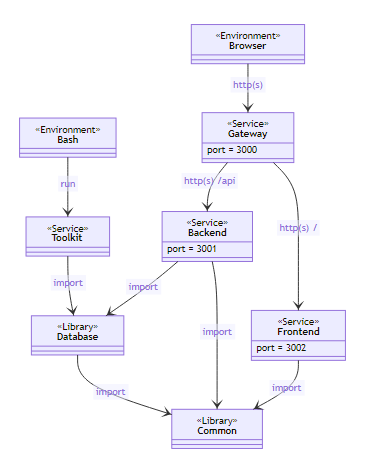
\includegraphics[width=\columnwidth]{packages-v3.png}
        \caption{Packages}
        \label{fig: packages}
    \end{figure}

    \subsubsection*{Gateway}
    The gateway runs at port 3000. It establishes a connection between the services backend, broker, worker and frontend. When the app is started the gateway serves as the entry address. It displays the frontend, which itself runs on port 3003, while the other services are running in parallel. To provide this functionality the gateway uses the express and the proxy library.  
  
    \subsubsection*{Frontend}
    The frontend provides an interface to make changes to the data via the offered functions of the developed API. To create the user interface React version 17 was used. It uses React states that can be altered with React hooks. The frontend communicates via HTTP requests with the backend to create, read, update and delete data with help of the API located in the backend. This communication runs with the library Axios. To display the uploaded cad models three.js was used. It offers a 3d view of the selected cad file. The view of the model can be adjusted by zooming and rotating, as well as positioning [see Fig. \ref{fig: versionview} on page~\pageref{fig: versionview}]. The library Recharts provides a variety of different charts and graphs. Recharts is used to display a burn down chart in a specific user interface component [see Fig. \ref{fig: sprintview} on page~\pageref{fig: sprintview}].

    \subsubsection*{Backend}
    The backend of the app is built with the framework nest.js. This area of the software is the core component and provides those functions to meet the previously defined requirement specifications. Using nest.js, an API was created that interacts with the data using CRUD commands and sends it to the frontend. For that, it receives commands from the frontend and then executes the corresponding function of the API. The backend is controlled via HTTP requests. Therefore, the commands can be executed without the frontend. Good possibilities are offered by the program Postman or with Swagger. A Swagger integration was done in the backend during the development process. Swagger provides good documentation about the API and allows its functions to be executed without the frontend.

    \subsubsection*{Common}
    The package common provides the necessary interfaces for the communication of the frontend and backend. In this section the data classes like product, version, issue, etc. for the different functions are defined. 
    The rest file contains the interfaces for the HTTP requests. They define exactly which data may be sent from the frontend and which may be received again. For this purpose, the CRUD methods with transfer parameter and return value are defined in each interface of a data class.
    
    \subsubsection*{Database}
    To store the data permanently a PostgreSQL database is used. It runs in a Docker container on port 5432. The database uses the data classes defined in the interface as entities. For the object relational mapping TypeORM is used. 
    
    \subsubsection*{Toolkit}
    The toolkit package provides functionality to fill the database with test data. Based on the classes defined in the interface, the respective objects are instantiated here. These objects are filled with fictitious data to test the functionality of the app. After the objects are instantiated, they are loaded into the database. For this purpose asynchronous function calls are executed.
    
    % \subsubsection*{Worker}
    % This package is not used yet. It is used to parallelize processes for later extensions of the software.
    
    % \subsubsection*{Broker}
    % This package is not used yet. It is used to send routing messages between different services for later extensions of the software.

    \subsection*{Data model}
    The core of the software is in the backend. Via the API, the data can be manipulated using CRUD methods. This section describes the data model of the app. The necessary classes and entities are based on the interfaces in the common package. The difference between the data in the backend and in the database is that each entity class in the backend is divided into update, add and the base class. In the database, the classes are not divided. For example, the class product is mapped to a table in the database.
    
    \subsubsection*{Entities}
    The data model contains the entities [see Fig. \ref{fig: erDiagram} on page~\pageref{fig: erDiagram}]:
    \begin{itemize}
        \item User
        \item Product
        \item Version
        \item Issue
        \item Comment
        \item Milestone
        \item Member
    \end{itemize}

    The primary key of each entity is its Id. At the top level of the data model is the user, who can create multiple products if he has the permission to do so. For each product versions, issues, comments, milestones and members can be created. The entity User has personal attributes like the profile picture name, email, password and the two permissions to create and change users or to create products. Finally, like any other entity, the user has a deleted flag. If a delete method is executed, this is set to true. The find and get methods of the API are implemented to search only for objects that are not deleted. When deleting, care must be taken which dependencies must also be set to deleted. If a user is deleted, no further data is removed from him. The user is only marked as deleted on the user interface. All data generated by the user will remain. All other entities are linked to the product entity. The product itself does not provide much information, because it will be filled with information later by other references. If a product is deleted, all versions, issues, comments, milestones, and members must also be set to deleted. The versions contain important information and the 3D CAD model. To create a versioning, the attributes major, minor and patch are specified for a version. the baseVersionIds are used to identify the previous version. By knowing the current version and previous version, a graphical overview can be built on the UI. Multiple issues can be added for each project. Label and text contain information about the issue. The state distinguishes between open and closed issues. So it is possible to filter for completed and not completed issues. The attribute assigneeId is a string array. Here the userIds of the users are specified who have the task to solve the issue. The milestoneId can be used to add the issue to a milestone. For each issue one or more comments can be created. These comments have a text, an author and a corresponding issue as well as the time of the post. With the attribute action an issue can be closed or reopened by the comment. For each product one or more milestones can be defined. These have a label and clear start and end dates. UserId and productId serve as foreign keys. Later it can be counted how many issues per milestone are still open or already closed. This can be used to display a graphical representation of the project progress in the frontend. For each product one or more members can be added. These members have the foreign keys productId and userId. The attribute role can have three states: manager, engineer, customer. Depending on the role, the corresponding product member has different permissions to interact with the respective product.

    \subsubsection*{Class diagram}
    The following figure [see Fig. \ref{fig: classdiagram} on page~\pageref{fig: classdiagram}] shows the data model of the developed API in the backend. In order to clearly define which data of a class is changed, added and constant, each class is divided into three subclasses that inherit from each other. Thus, the classes are divided into UpdateData, AddData and the entity itself. AddData inherits from UpdateData and the Entity inherits again from AddData. The respective Entity subclasses serve as passing parameters for the API methods. Each entity has an ID as primary key and a deleted attribute. The find methods of the API are defined in such a way that they return only objects, where the deleted attribute is false. So if data is deleted, it is only marked with a deleted flag and will not be found again. If data is created, then the necessary references are generated, such as the associated product or the selected user. These attributes are comparable with foreign keys and are located in the AddData classes. The UpdateData classes contain attributes of the respective entity, which can be changed by the API in the later course. 

    \begin{figure*}[t]
        \centering
        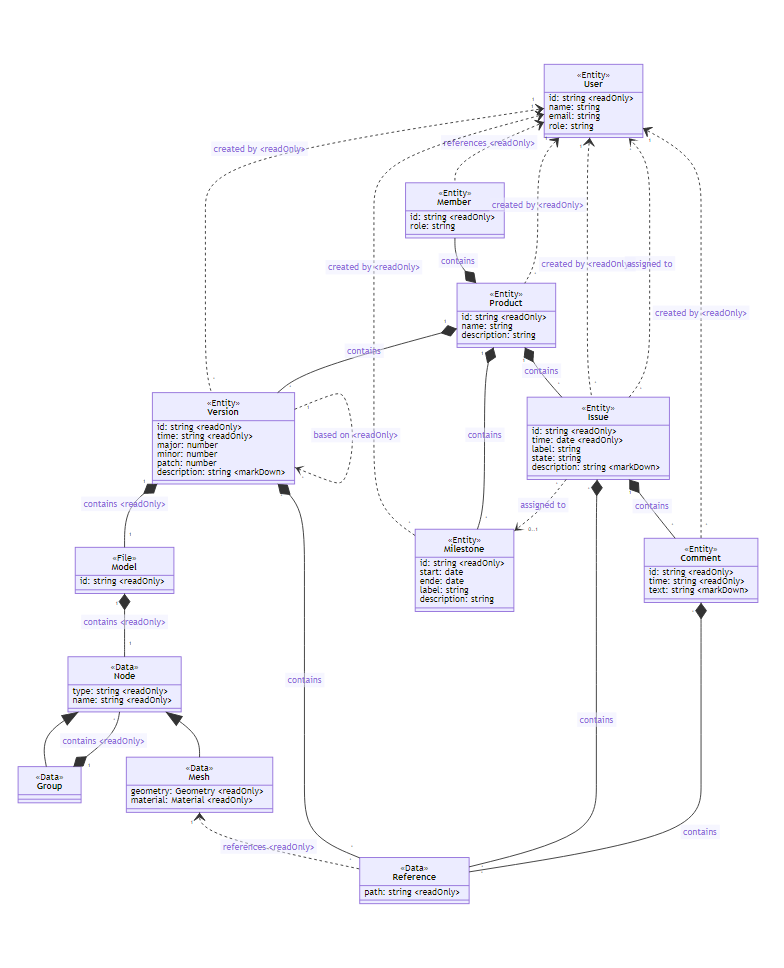
\includegraphics[width=\textwidth]{entities-v5.png}
        \caption{Data model}
        \label{fig: classdiagram}
    \end{figure*}

    \subsubsection*{Entity relationship diagram} % optional o machen im diagram
    The entity-relationship model [see Fig. \ref{fig: erDiagram} on page~\pageref{fig: erDiagram}] has a simpler structure like the class diagram. It consists of the exact entities that are used in the interface and API. Since this is only the data store, the classes are not structured in three subclasses. One table is reserved in the database for the entire object. Since the objects of the API and the database are not identical, these must be converted with each write and read process. The database entities are mapped to tables with TypeORM. 

    \begin{figure*}[t]
        \centering
        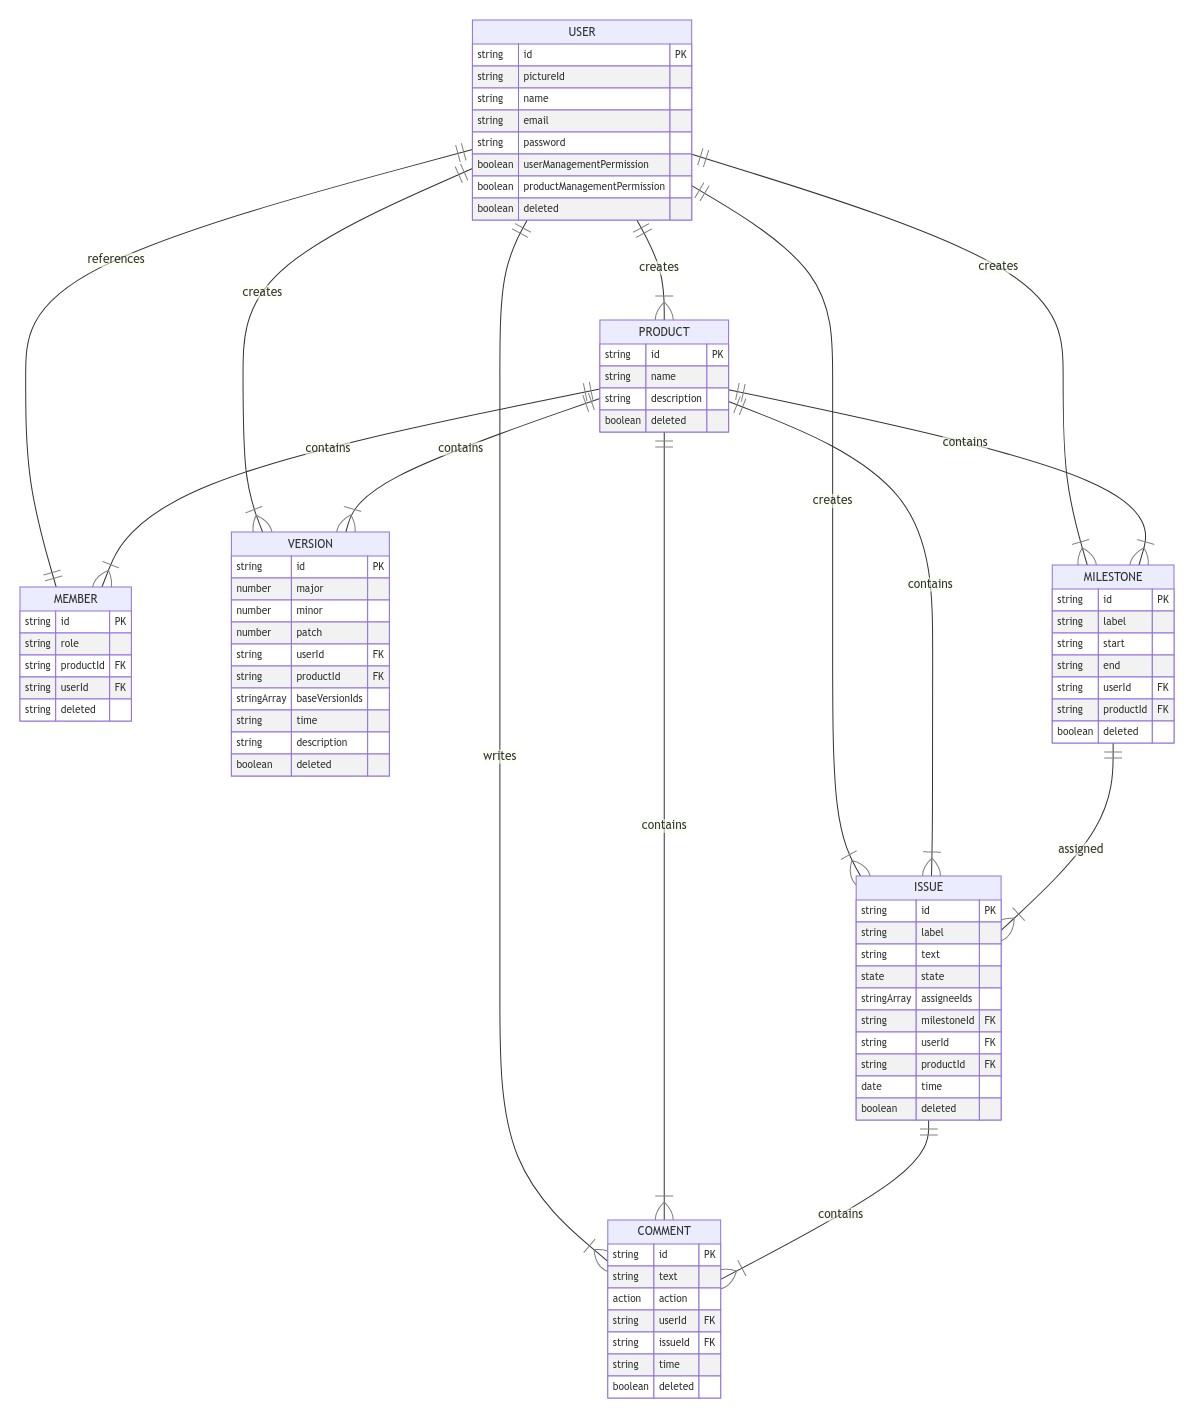
\includegraphics[width=\textwidth]{erDiagram-v1.png}
        \caption{Entity relationship diagram}
        \label{fig: erDiagram}
    \end{figure*}

    \subsection*{Function model} 
    The functions implemented in the API allows to create, read, update and delete data. This would not even require a graphical user interface. All functions offered by the API are called via HTTP requests. These requests can also be made via the console or other software such as Postman or Swagger. Thus, the functional model in combination with the data model is the foundation of this application. The API is built with nest.js. One rest entity contains of controller, service and module. In operation, an HTTP request is performed in the frontend. The data flows from the respective view via a request manager to a rest method, where the respective Axios request is triggered. In the backend, the nest controller receives the request and sends it on to the nest service. The nest service implements the necessary API methods to make changes to the data. These functions are all asynchronous and have a Promise as return value. After processing, the result is returned. This tunnel is provided with various permission checks to verify that the user or product member has the permission to perform this action. The interface in the common package controls the communication between frontend and backend. In the nest service the methods find, add, get, update, delete and convert are available. The convert method parses the received database object back into an object that can be further processed by the software.

    \subsubsection*{User management}
    Users can be created, modified and deleted here. The condition for this is that the respective user has the User Manager Permission. When a user is created, the associated data object is filled with the respective attributes. Permissions can be assigned to allow the new user to create and edit other users and to create products. For this the two attributes user management permission and product management permission have been added. The API offers the following methods for interaction with user objects:
    
    \begin{itemize}
        \item findUsers(query?: string, productId?: string) 
        \item addUser(data: UserAddData, file?: File)
        \item getUser(id: string)
        \item updateUser(id: string, data: UserUpdateData, file?: File)
        \item deleteUser(id: string)
    \end{itemize}

    The \texttt{findUsers} method searches for all users of the system from the database. It can be searched either via a query by user name or via the product id. The parameters query and productId are optional. Depending on which parameter is specified, the search process runs differently. The users found in the database are converted into user objects with the convert method, pushed into an array and returned. For the addUser method the transfer parameter is needed, which contains the information about the new user. The second parameter holds the profile picture and is optional. The UserAddData object is generated in normal operation via the User settings view and sent to the backend. GetUser searches for a specific user based on the userId and returns the object after conversion. UpdateUser needs the userId, the UserUpdateData object and optionally a file containing a profile picture. DeleteUser sets the deleted flag of the particular user to true. The get and find methods are implemented that way, to search for objects that are not deleted. The convert method is in each class and parses the database entities back into objects for further processing.

    \subsubsection*{Product management}
    This part of the API provides methods to make modifications to product objects. Here products can be created, modified and deleted. The following bullet points show the methods that are available for interacting with products:

    \begin{itemize}
        \item findProducts()
        \item addProduct(data: ProductAddData)
        \item getProduct(id: string)
        \item updateProduct(id: string, data: ProductUpdateData)
        \item deleteProduct(id: string)
        \item convert(user: ProductEntity)
    \end{itemize}

    The findProducts method searches in the database for all products that are not deleted. For this no passing parameter is necessary. The other methods work according to the same principle as in user management. It is searched with the corresponding productId for the object and displayed or its properties get changed. When deleting a product, it must be ensured that all objects that are attached to a product are also deleted. So if a product is deleted, all versions, issues, milestones and members must also be set to deleted.

    \subsubsection*{Version management}
    Only by referencing a version to a product it gets further descriptive properties and the 3D CAD model. Again, the API provides CRUD methods to interact with versions:

    \begin{itemize}
        \item findVersions(productId: string)
        \item addVersion(data: VersionAddData, file: File)
        \item getVersion(id: string)
        \item updateVersion(id: string, data: VersionUpdateData, file?: File)
        \item deleteVersion(id: string)
        \item convert(user: VersionEntity)
    \end{itemize}

    Unlike user management, a file must be specified when a version is created. This is an STL file, which is then stored locally. This CAD model can be exchanged when updating the version.

    \subsubsection*{Issue management} 
    These methods are available to create, read, update and delete issues:
    \begin{itemize}
        \item findIssues(productId: string, milestoneId?: string, state?: 'open' or 'closed')
        \item addIssue(data: IssueAddData)
        \item getIssue(id: string)
        \item updateIssue(id: string, data: IssueUpdateData)
        \item deleteIssue(id: string)
        \item convert(user: IssueEntity)
    \end{itemize}

    The findIssues method can search for issues in the database in several ways. An issue is always connected to a product. Thus, the productId must always be passed. Aditionally, the milestoneId parameters can be given to the method to search for issues that belongs to a specific milestone. The state parameter allows to filter the issues by closed and open. This is especially useful to be able to filter for completed or uncompleted tasks for  the purpose of product management. When deleting issues, all comments belonging to the respective issue must also be deleted.

    \subsubsection*{Comment management}
    % comments select parts Datenmodell
    The following list shows the methods that can be performed to interact with the comment objects:
    \begin{itemize}
        \item findComments(issueId: string)
        \item addComment(data: CommentAddData)
        \item getComment(id: string)
        \item updateComment(id: string, data: CommentUpdateData)
        \item deleteComment(id: string)
        \item convert(user: CommentEntity)
    \end{itemize}

    An issue can have one or more comments. These comments are bound to an issue and the issue is bound to a product. The findComments method stores all comments for a given issueId in an array and returns it. 

    \subsubsection*{Milestone management}
    Milestones are a container that can be filled with issues by reference. The CRUD methods are listed below:
    \begin{itemize}
        \item findMilestones(productId: string)
        \item addMilestone(data: MilestoneAddData)
        \item getMilestone(id: string)
        \item updateMilestone(id: string, data: MilestoneUpdateData)
        \item deleteMilestone(id: string)
        \item convert(user: MilestoneEntity)
    \end{itemize}

    The methods have analogous purposes as already with the other data objects. When deleting a milestone, it must be ensured that the references to the linked issues are removed. For this purpose, the milestoneId attribute of each associated issue is set to null again.

    \subsubsection*{Member management}
    The API provides the following methods for member management:

    \begin{itemize}
        \item findMembers(productId: string, userId?: string)
        \item addMember(data: MemberAddData)
        \item getMember(id: string)
        \item updateMember(id: string, data: MemberUpdateData)
        \item deleteMember(id: string)
        \item convert(user: MemberEntity)
    \end{itemize}

    Members are always linked to the respective product. Additionally, the userId can be used to search for one specific member. The findMembers method returns an array of members that can then be displayed on the user interface.
    The other methods are similar to those of the other entities

    \subsection*{Permission model}
    The permission model offers a number of possible restrictions on the platform so that not every user has all freedoms. This is especially important when cooperating with customers. The customer should only have the possibility to evaluate existing products. For this he can see the products he is registered for and use the given product management functions. Creating new users and products should only be possible by the developers of the respective product. They also organize the rights of each user. The permission model is divided into two levels. The first level is the user level and the second level is created by the product members. This system is deeply integrated in the backend. Each method of the API checks with each call whether the respective user or the member role has the necessary permissions for the execution. All permission of the respective user and member roles are stored in a separate permissions.ts file. 

    \subsubsection*{User level}
    The User entity has the two attributes user management permission and product management permission. Only a user who has the user management permission can see the Users button in the upper right corner of the frontend and create or edit users there. With the product management permission it is possible to create new products. If a new product is created, the respective user is automatically also a product member and receives the member role manager. The permissions of each user can be adjusted afterwards in the user settings [see Fig. \ref{fig: usersettingsview} on page~\pageref{fig: usersettingsview}]. So it is possible to give multiple users the permissions for user administration and product administration. For example, a user and product manager can exist for each department The following table [see Fig. \ref{tab: userlevelpermissions} on page~\pageref{tab: userlevelpermissions}] shows the division of permissions into user management and product management on user level.

    \begin{figure}[h]
        \centering
        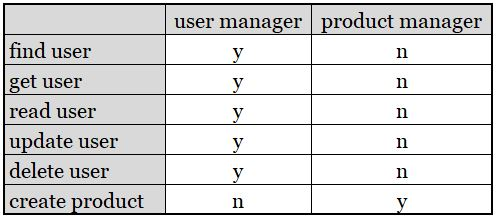
\includegraphics[width=7cm]{userlevelpermissions.JPG}
        \caption{Permissions on user level}
        \label{tab: userlevelpermissions}
    \end{figure}

    \subsubsection*{Member level}
    For permission management at member level, three roles are provided. These roles are: manager, engineer and customer. The manager is the one who created the product and has the permission to add more members. So he can add more managers, who in turn have all the rights over the management of the product. This is useful when the product development covers several departments. The second role is the engineer. He is involved in the product development process. He has no rights to change the product or its members. However, he can freely create and edit versions, issues, comments and milestones. The last role is the customer who has the possibility to observe the product development process. He can follow the progress of the project, but has no permission to change anything on the platform. In the current version of the software the rights of the customer are still very strict. The permission system is implemented in such a way that it can be changed with few adjustments. If the customer needs writing permissions, this can be easily changed in the code. For this purpose, there is a separate file in the backend, which implements exactly these two tables for the permission management. The corresponding table [see Fig. \ref{tab: memberlevelpermissions} on page~\pageref{tab: memberlevelpermissions}]  shows an overview of the respective permissions on member level.

    \begin{figure}[h]
        \centering
        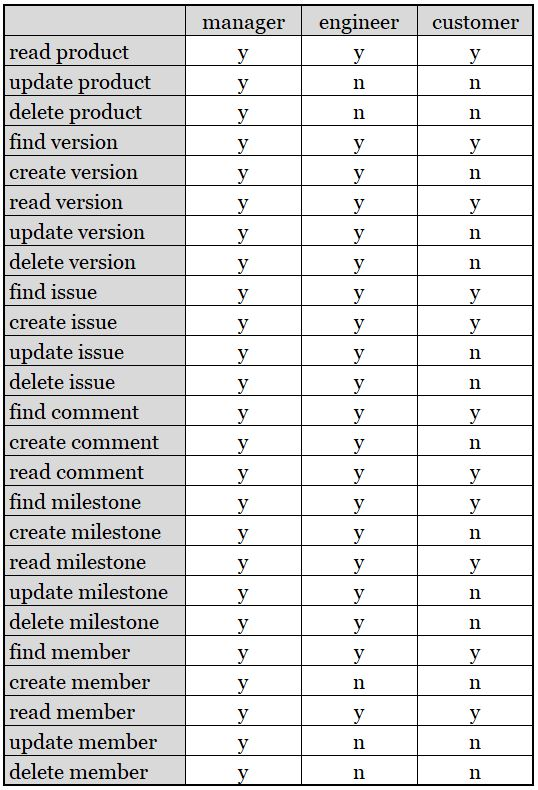
\includegraphics[width=7cm]{memberlevelpermissions.JPG}
        \caption{Permissions on member level}
        \label{tab: memberlevelpermissions}
    \end{figure}
    
    \subsection*{Interface model} 
    The user interface provides a convenient way to interact with the functional model to modify and display data. For the frontend the library React.js version 17 was used. The data is managed in react states and manipulated with react hooks. Typescript was used for programming. The pages were designed with simple CSS without additional tools. The user interface offers a consistent design, which runs through the entire system. The header of the user interface offers three buttons. A click on ProductBoard leads back to the start page. On the right side there is the user administration and the currently logged-in user. The button to view the users is only visible if the current user has the user management permission. The rest of the page below the header adapts to the corresponding content.

    \subsubsection*{Start page}
    After a successful login with username and password you will see the start page. This page lists all available products in a table [see Fig. \ref{fig: startpage} on page~\pageref{fig: startpage}]. For each product in the table a preview is shown. The other columns show the attributes Owner, Name, Description, Versions, Issues and Members. The X on the right provides the possibility to delete the corresponding product. The owner is the person who created the product. Name and Description are defined when the product is created and can be changed later in the Product Settings [see Fig. \ref{fig: productsettingsview} on page~\pageref{fig: productsettingsview}]. The columns on the right show how many versions exist for this product, how many issues have been created and how many members have access to the product. By clicking on New product you get to a separate page where you can add a new product [see Fig. \ref{fig: newproductview} on page~\pageref{fig: newproductview}]. This button is only visible when the corresponding user has product management permission. After entering name and description the new product appears in the product list on the start page. Only by creating a new version for a product a CAD model with further information is added.

    \begin{figure}[h]
        \centering
        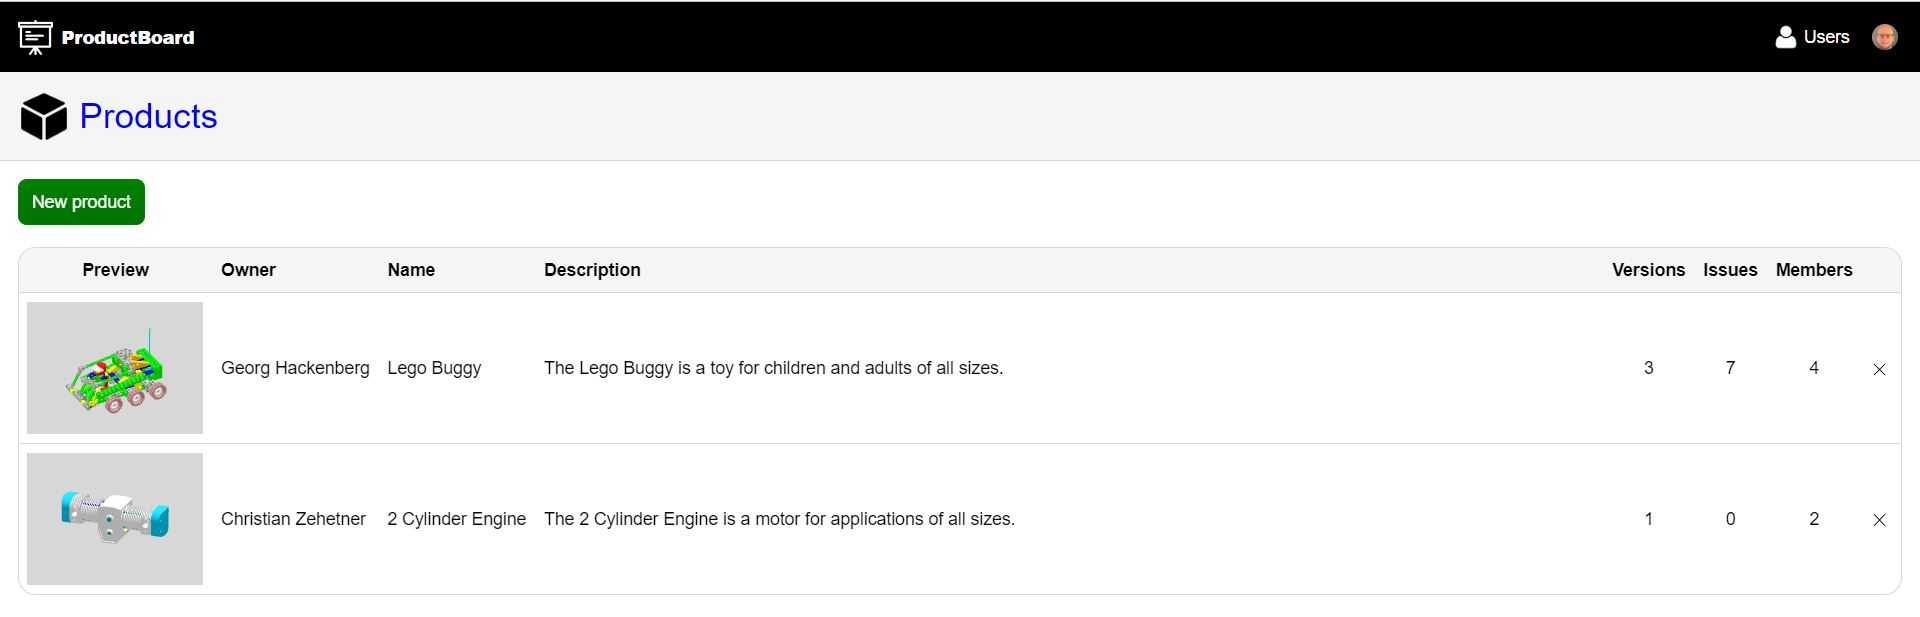
\includegraphics[width=7cm]{startpage.JPG}
        \caption{Startpage}
        \label{fig: startpage}
    \end{figure}

    \begin{figure}[h]
        \centering
        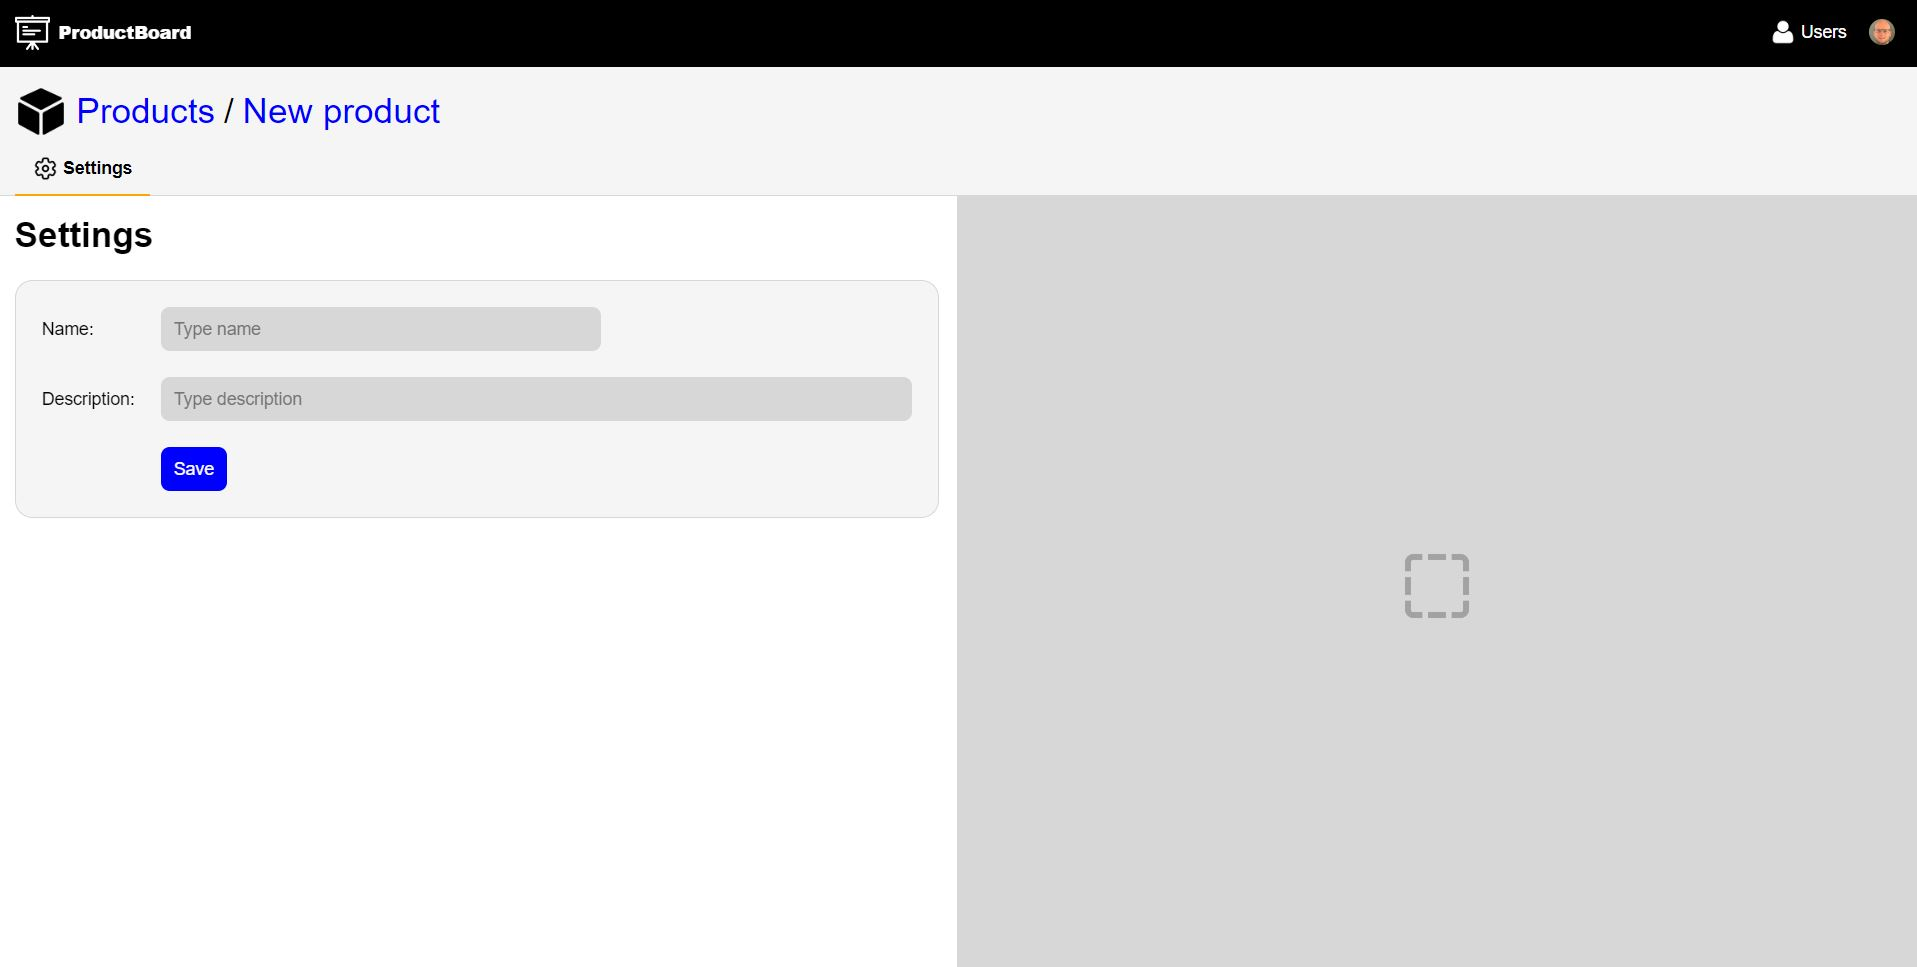
\includegraphics[width=7cm]{newproductview.JPG}
        \caption{Add new product}
        \label{fig: newproductview}
    \end{figure}

    \subsubsection*{User management}
    This view is only accessible if the active user also has the authorization. By clicking on Users this page is called. If the user does not have user management permission, the button is not visible. On this page all users with profile picture, name, email and permissions are displayed [see Fig. \ref{fig: usermanagement} on page~\pageref{fig: usermanagement}]. You can delete a user by clicking on the X on the right side. If a user is clicked on, he can be edited via the User settings. The button New user also leads to the user settings where you can provide information and create a new user by clicking on the save button [see Fig. \ref{fig: usersettingsview} on page~\pageref{fig: usersettingsview}]. Save leads back to the user overview and shows the new or changed user in the table.
    
    \begin{figure}[h]
        \centering
        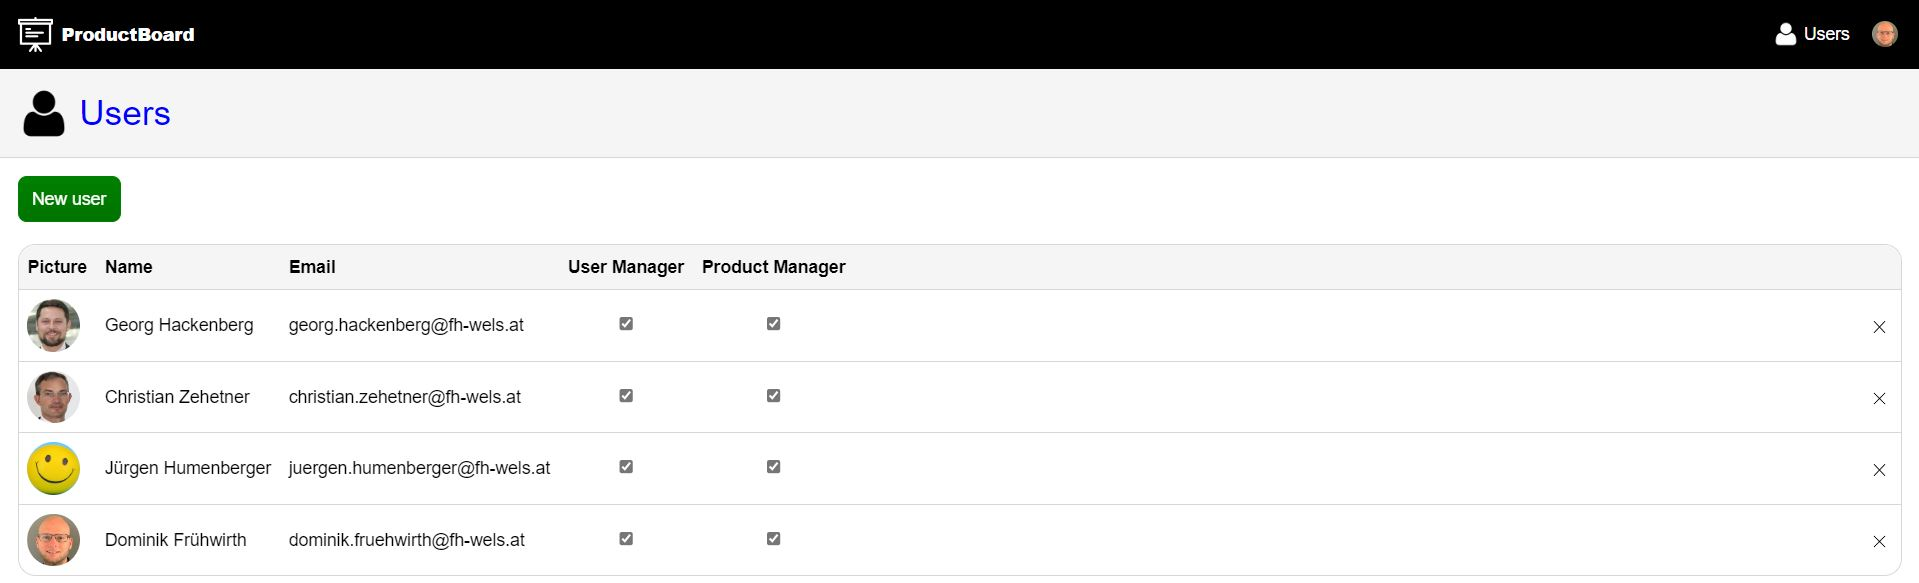
\includegraphics[width=7cm]{usermanagement.JPG}
        \caption{User management}
        \label{fig: usermanagement}
    \end{figure}

    \begin{figure}[h]
        \centering
        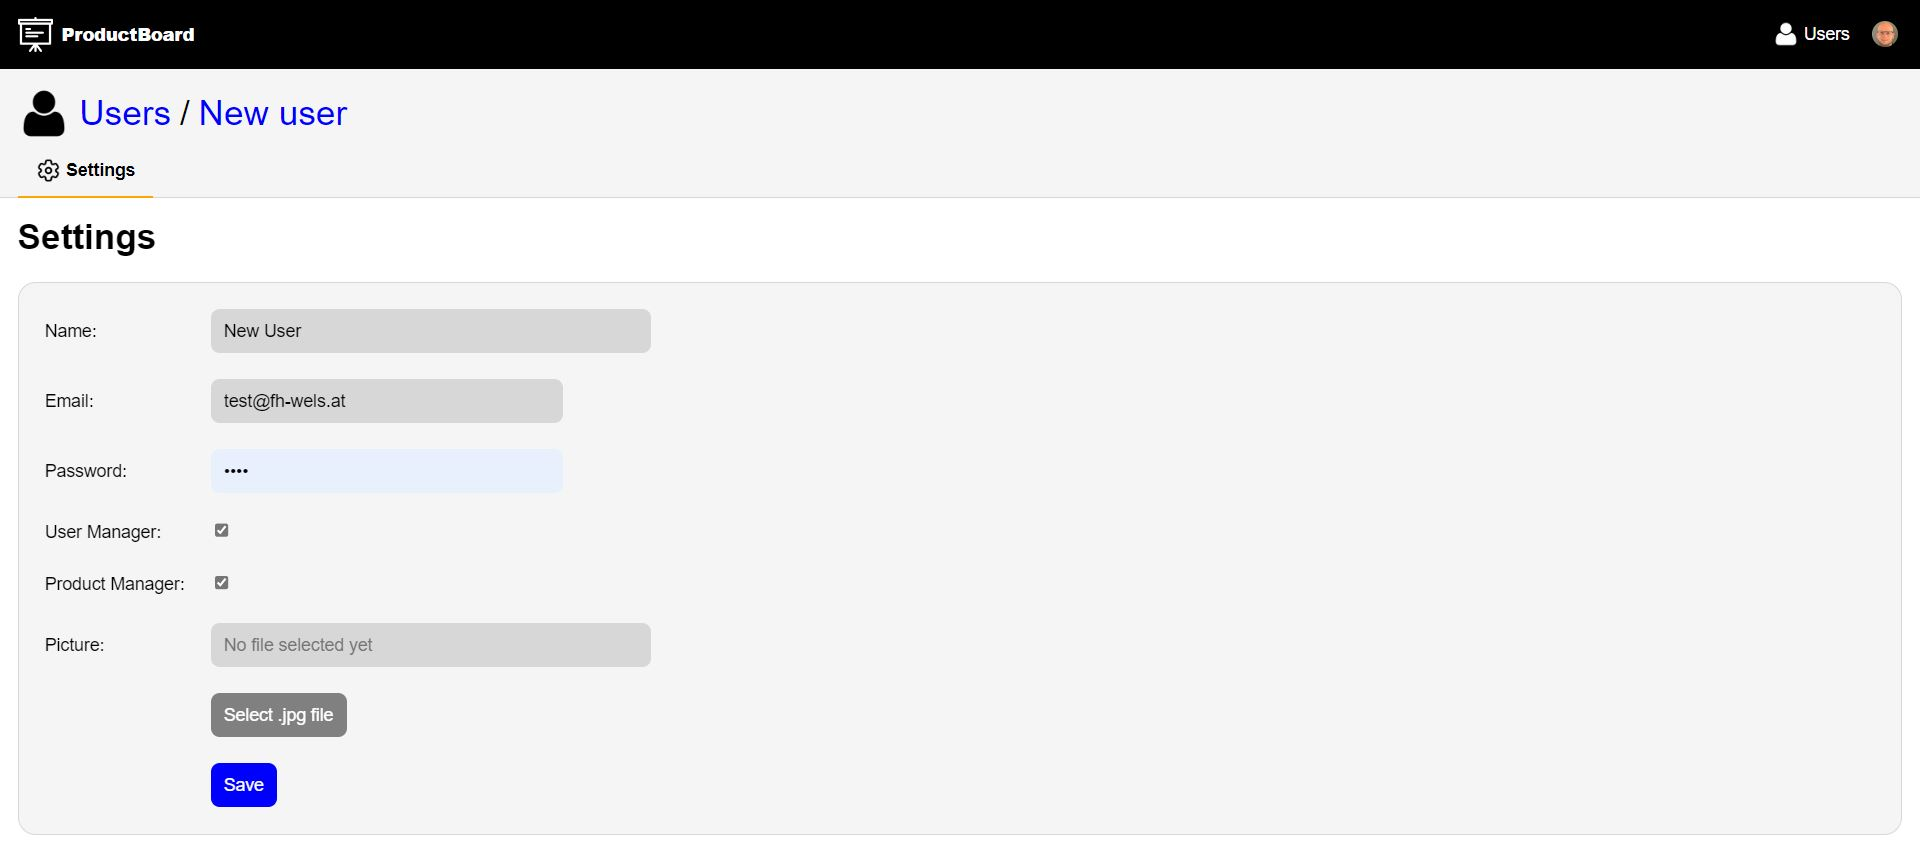
\includegraphics[width=7cm]{usersettingsview.JPG}
        \caption{User settings}
        \label{fig: usersettingsview}
    \end{figure}

    \subsubsection*{Version view}
    Clicking on a product takes you to the version view [see Fig. \ref{fig: versionview} on page~\pageref{fig: versionview}]. You can also use the toolbar to jump to other pages such as Issues, Milestones Members or Settings. Next to the links a number in brackets shows how many objects per category have already been created. The left side of the Version view shows the created versions. On the left side there is a tree structure similar to Git. In the middle is the corresponding version number with the owner of the version inclusive email and a short description. Each version offers a preview. By clicking on the respective version, the 3D view on the right side also changes and shows the selected model. The 3D view was built with three.js. It allows to rotate, move and zoom the model. With a click on New version you get to the version settings [see Fig. \ref{fig: versionsettingsview} on page~\pageref{fig: versionsettingsview}]. There you can enter information for a new version and select an STL file. Depending on the selected base version, the version view shows the new version with the corresponding new tree structure after pressing the Save button.
    
    \begin{figure}[h]
        \centering
        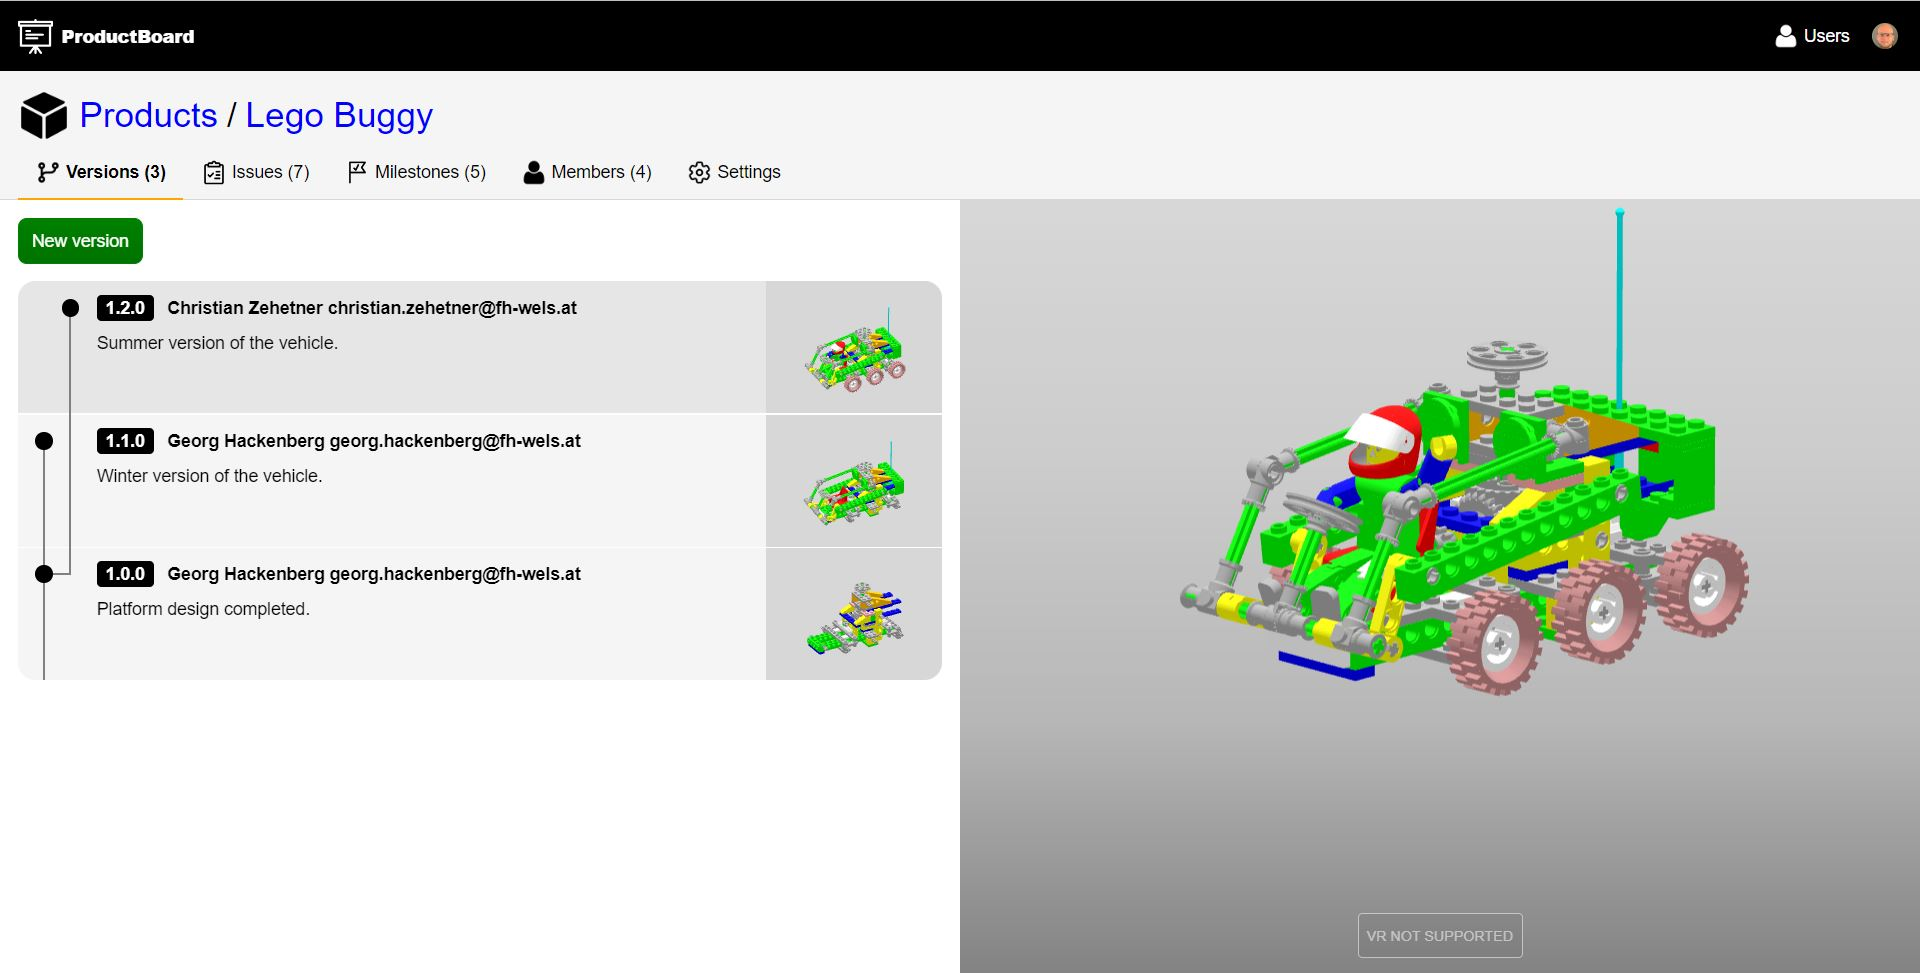
\includegraphics[width=7cm]{versionview.JPG}
        \caption{Version view}
        \label{fig: versionview}
    \end{figure}

    \begin{figure}[h]
        \centering
        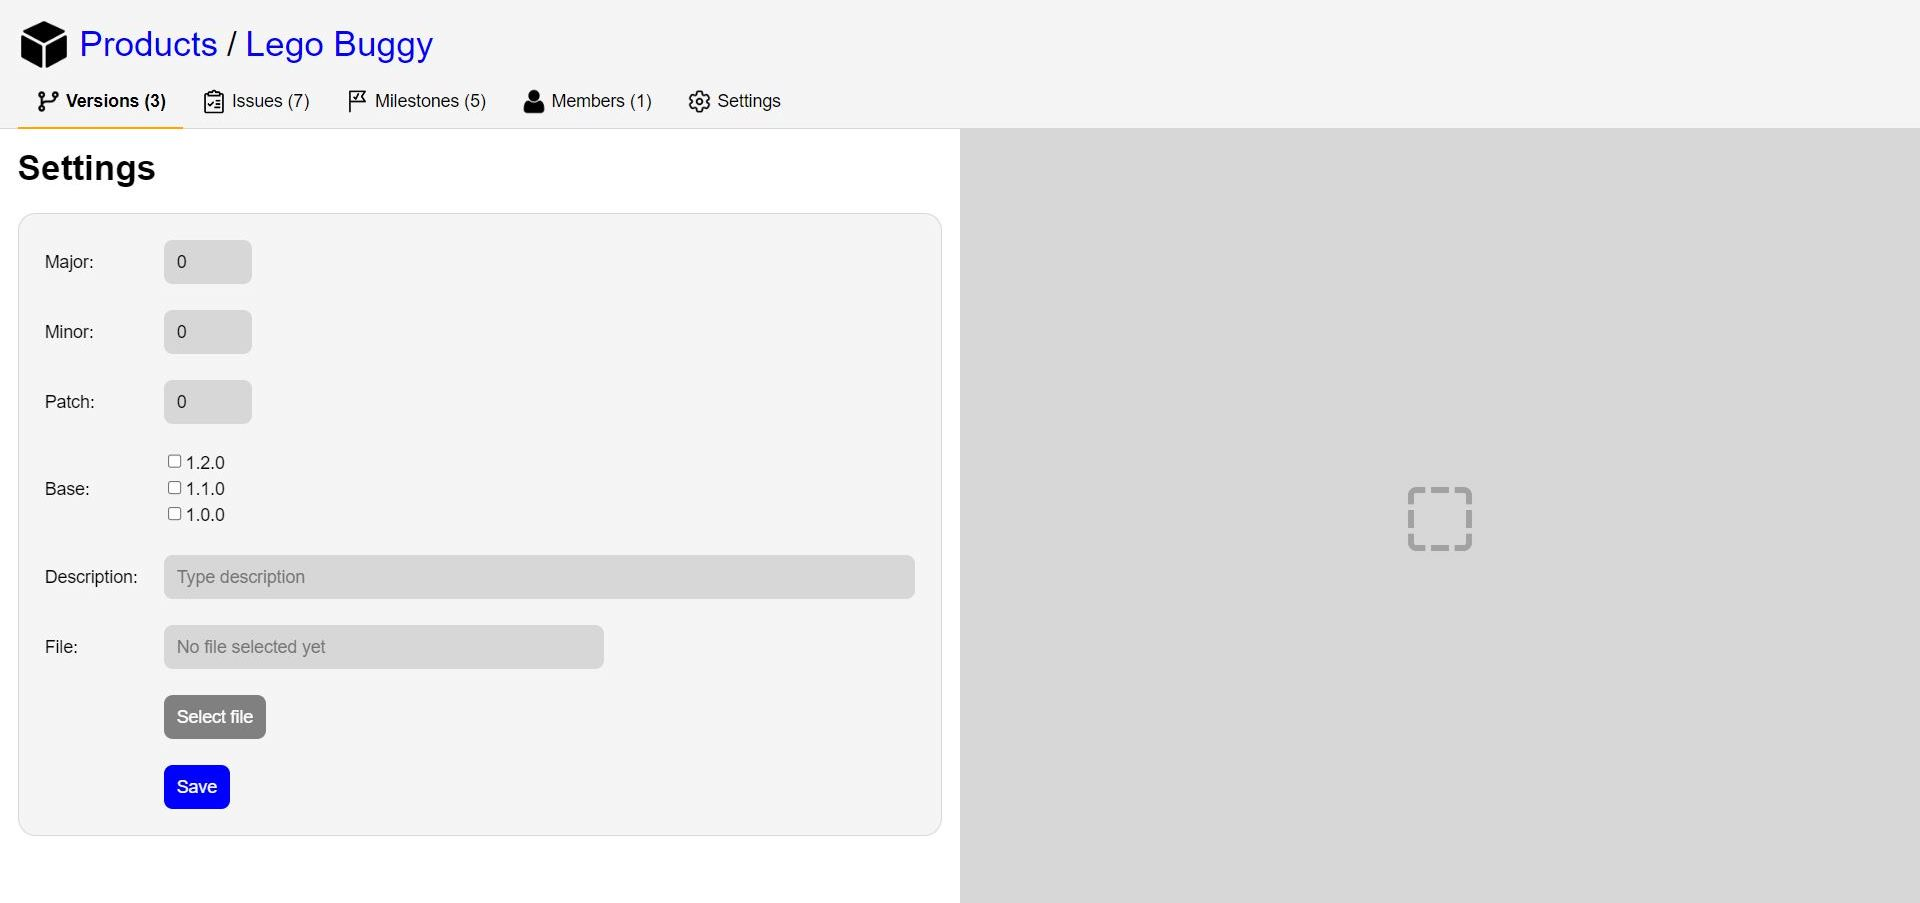
\includegraphics[width=7cm]{versionsettingsview.JPG}
        \caption{Versionsettings view}
        \label{fig: versionsettingsview}
    \end{figure}

    \subsubsection*{Issue view}
    By clicking on the Issues link, you access the Issue view [see Fig. \ref{fig: issueview} on page~\pageref{fig: issueview}]. Here the created issues are displayed in a table. The two buttons Open Issues and Closed Issues can be used to filter the list accordingly. The table shows the reporter who created the issue, the associated label, the assignees and how many comments and marked parts are in the conversation channel. The Issue settings view allows to create new issues for the product [see Fig. \ref{fig: issuesettingsview} on page~\pageref{fig: issuesettingsview}]. The label, the text, the milestone and the assignees can be defined. An existing milestone can be selected with the dropdown menu. An issue must not be assigned to a milestone. This choice lies by the user. The Save button closes the settings, and you return to the Issues view where the new issue is visible. All views with 3D View offer the possibility to select a desired version for viewing. In the version view the version can be clicked directly. In the other views the version can be selected via a dropdown menu. This menu is located in the upper left corner of the 3D View.
    
    \begin{figure}[h]
        \centering
        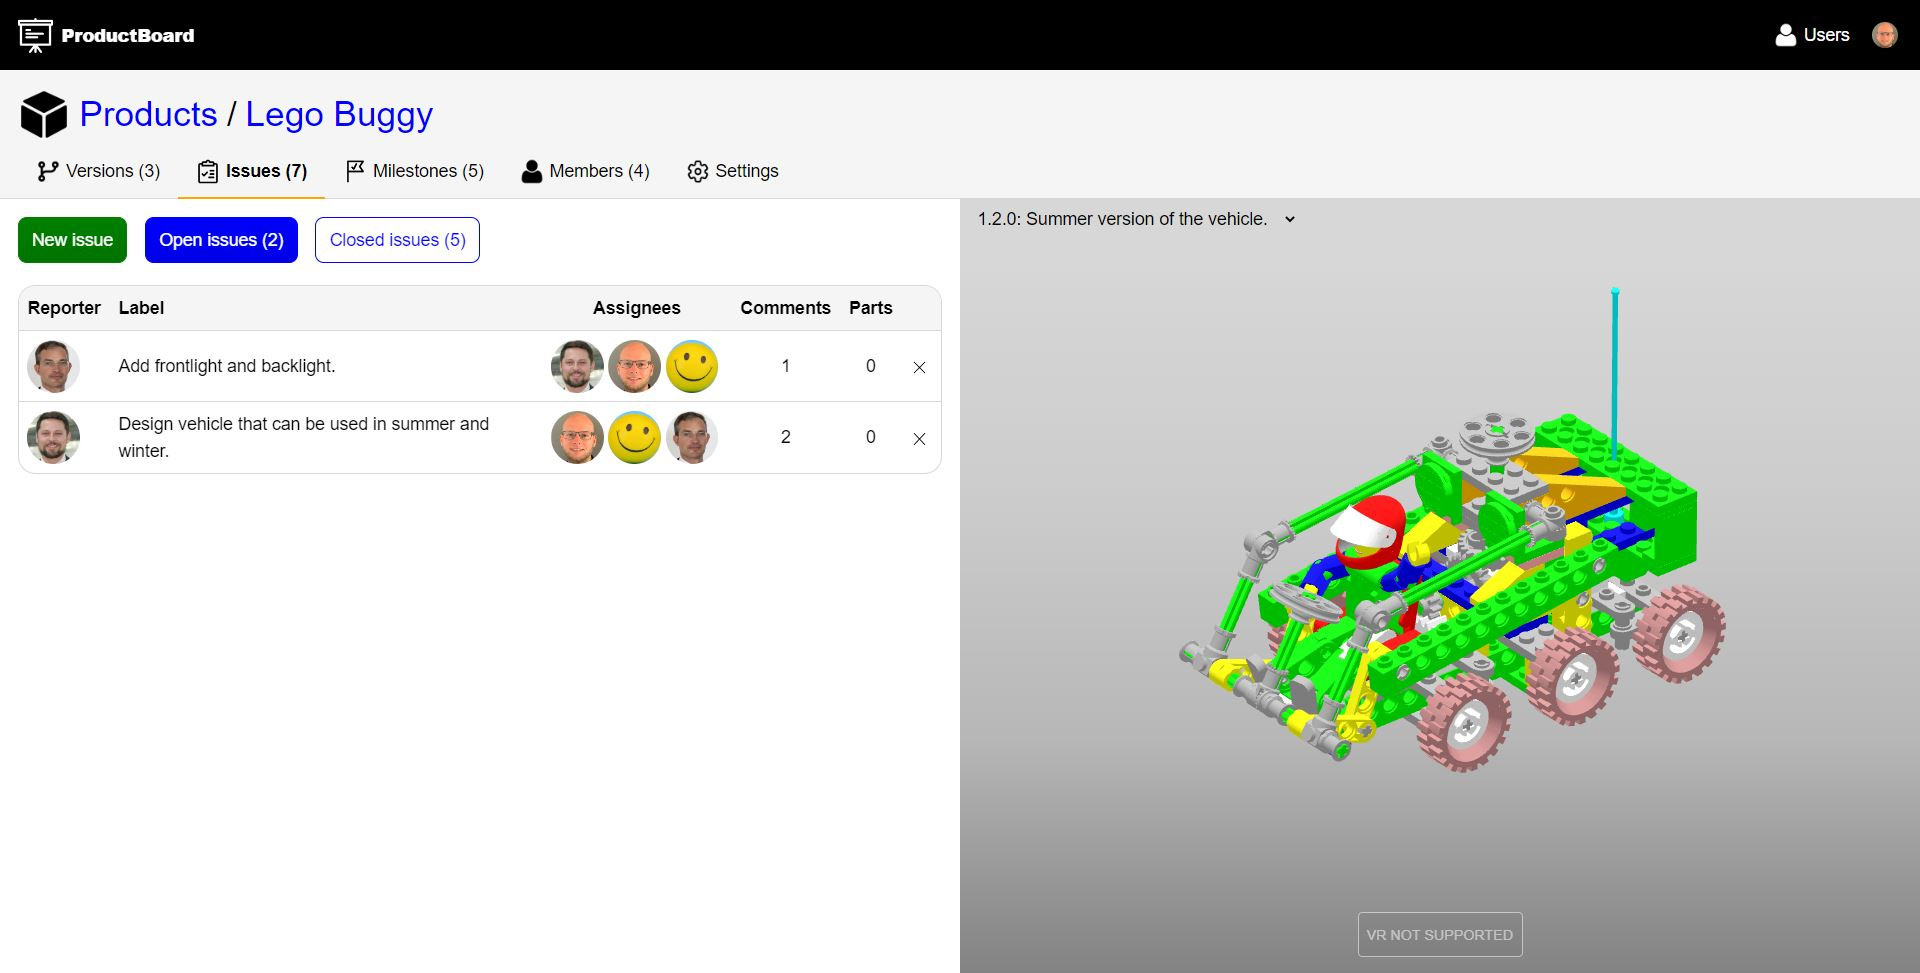
\includegraphics[width=7cm]{issueview.JPG}
        \caption{Issue view}
        \label{fig: issueview}
    \end{figure}

    \begin{figure}[h]
        \centering
        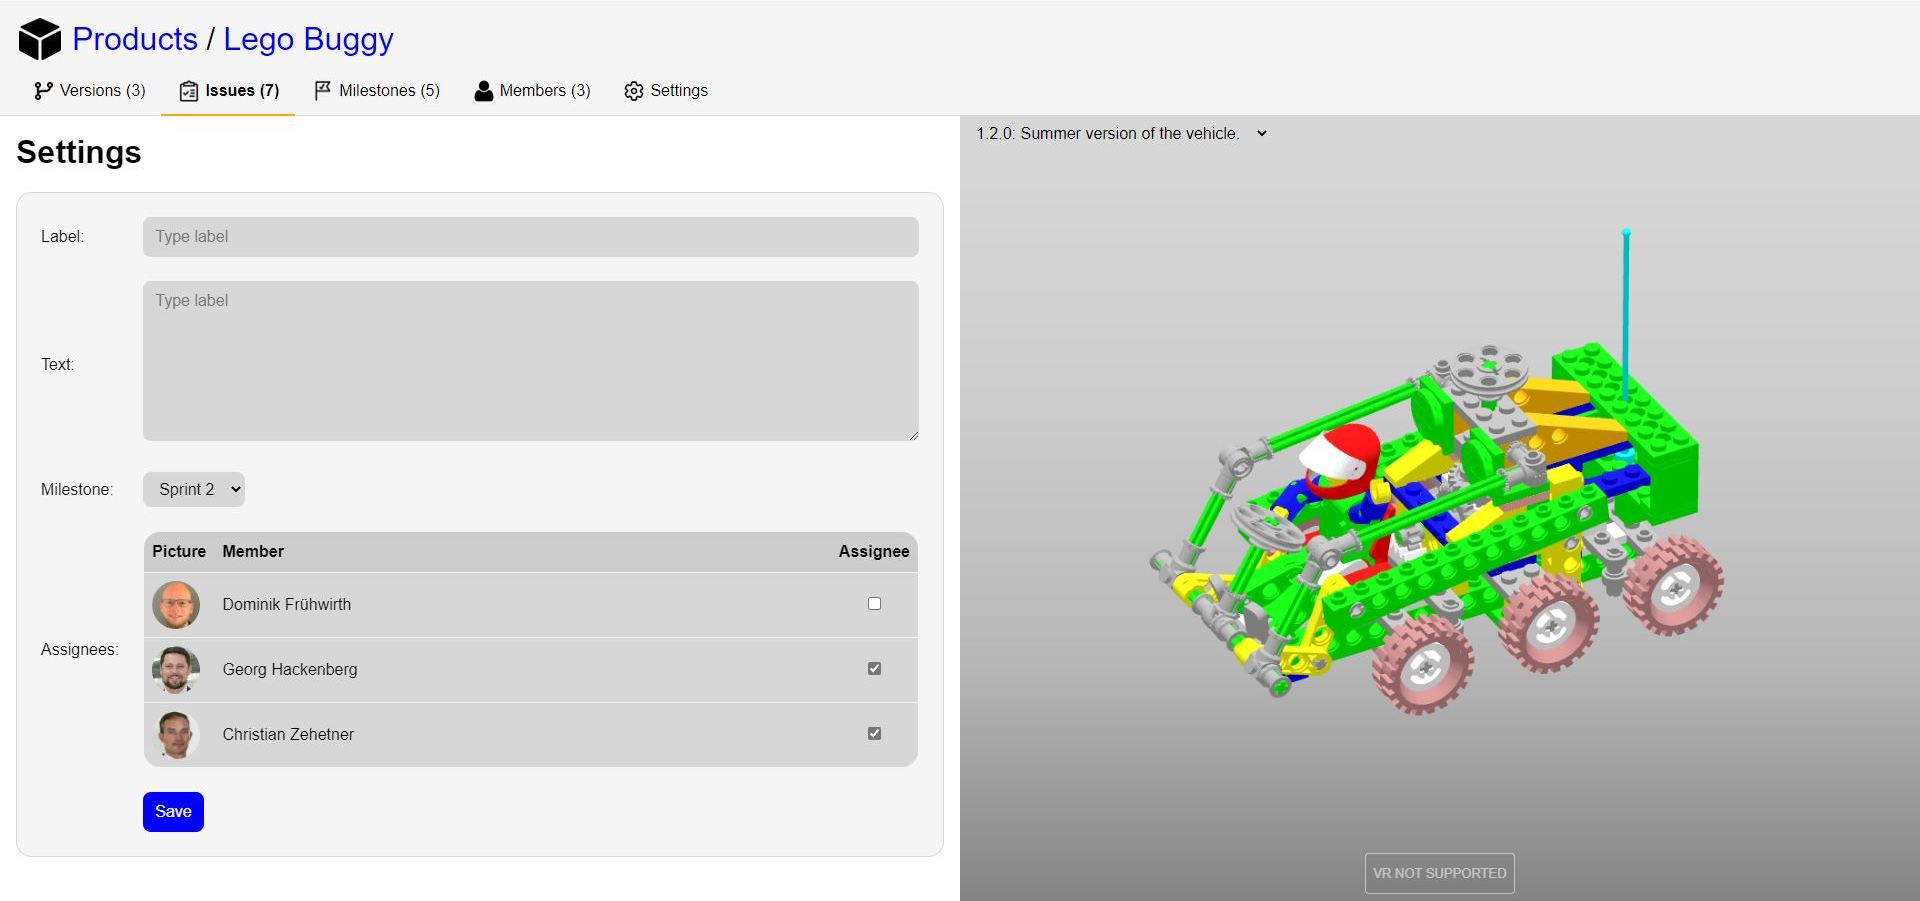
\includegraphics[width=7cm]{issuesettingsview.JPG}
        \caption{Issuesettings view}
        \label{fig: issuesettingsview}
    \end{figure}

    \subsubsection*{Comment view}
    Clicking on an issue in the Issue view opens the corresponding Comment view [see Fig. \ref{fig: commentview} on page~\pageref{fig: commentview}]. Here you have the possibility to discuss the issue. You can click on a component of the 3D model in the Comment view to reference a component [see Fig. \ref{fig: commentselectedpartview} on page~\pageref{fig: commentselectedpartview}]. If a post is created or a part is selected in the comment view, the corresponding counter in the issue view table is increased. A comment can be used to close an issue by clicking Close. This issue will then be found in Closed Issues in the Issue view. With the comment function it is also possible to reopen the issue in the same way. The Close button displays the text Reopen when an issue is closed. In the upper right corner of the Comment view there is a button to edit the selected issue. For example, the issue can be assigned to another Milestone or other attributes can be changed [see Fig. \ref{fig: issuesettingsview} on page~\pageref{fig: issuesettingsview}]. A click on Save makes the changes visible in the Issue view.

    \begin{figure}[h]
        \centering
        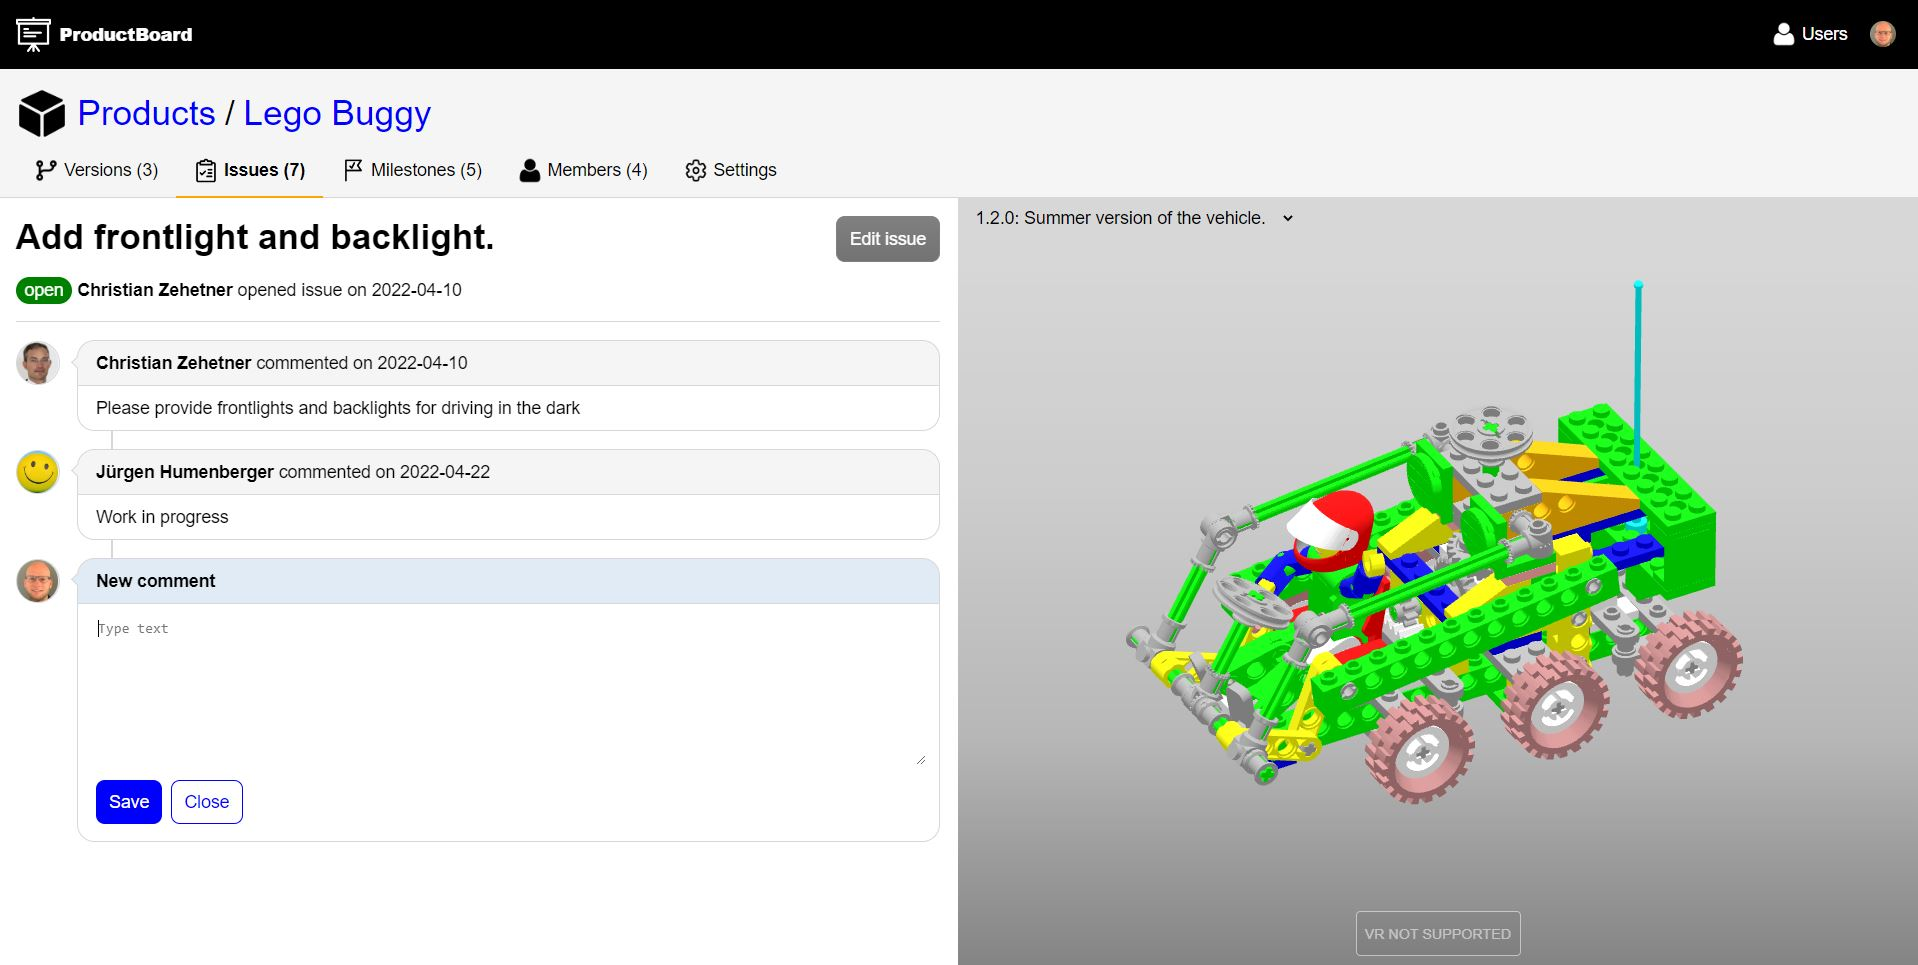
\includegraphics[width=7cm]{commentview.JPG}
        \caption{Comment view}
        \label{fig: commentview}
    \end{figure}

    \begin{figure}[h]
        \centering
        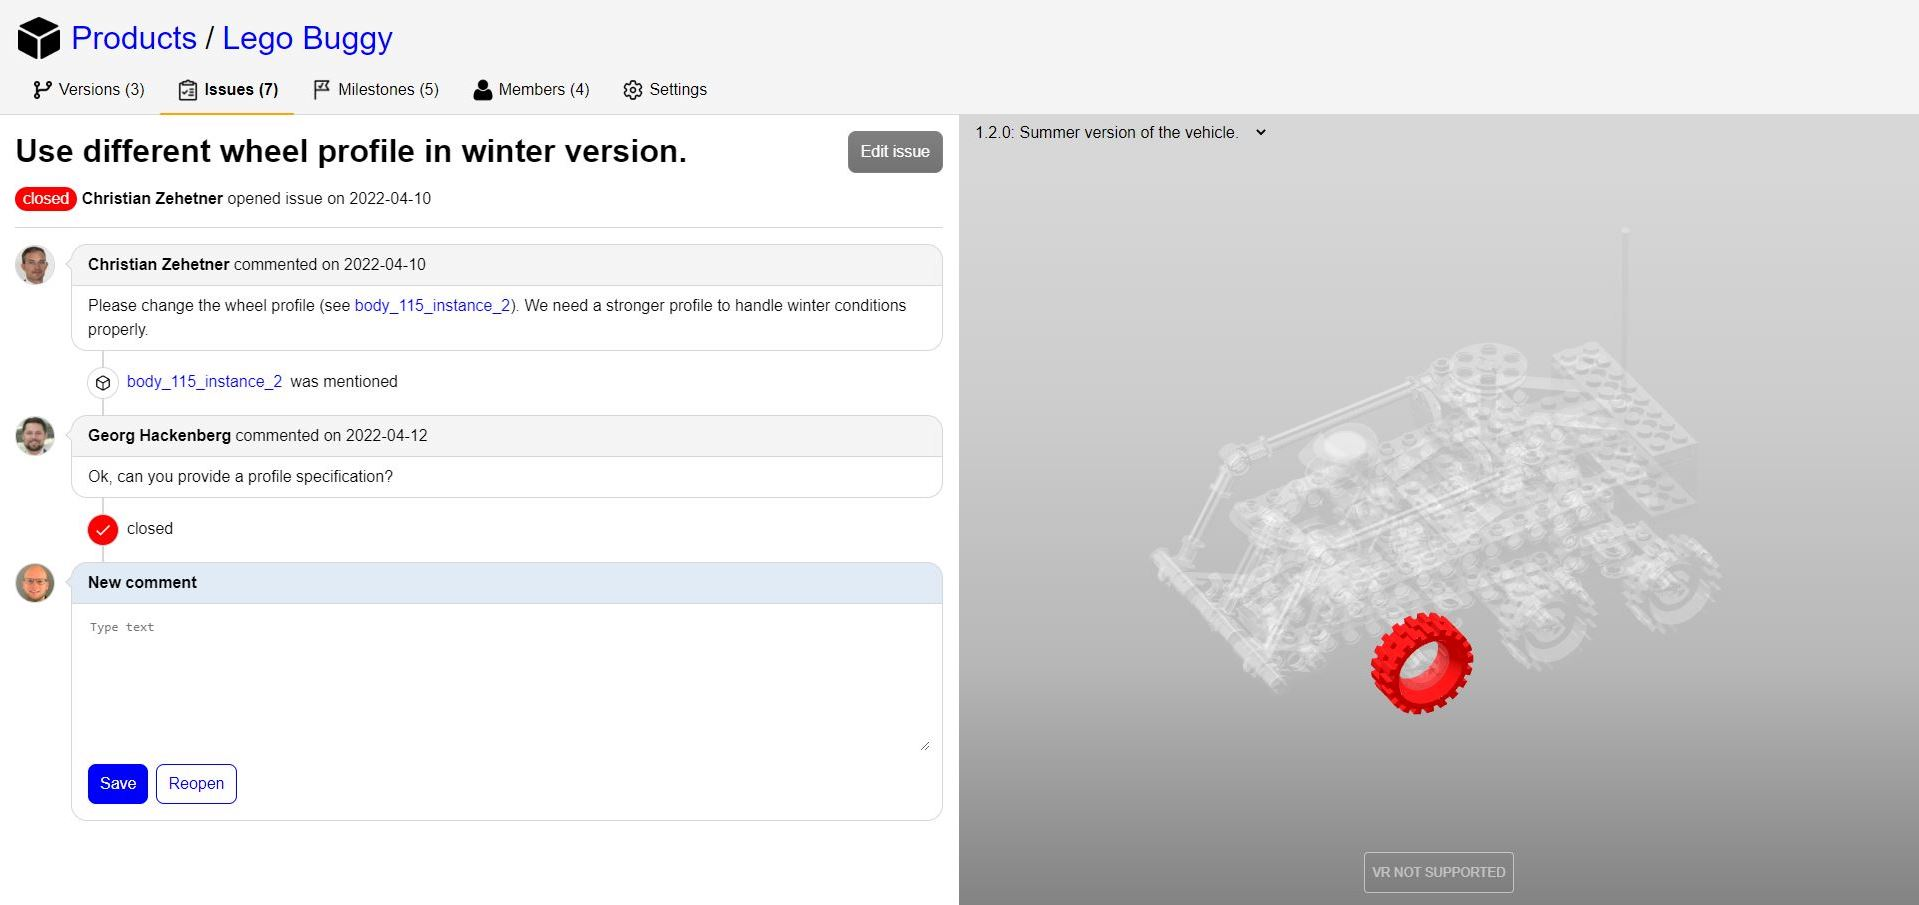
\includegraphics[width=7cm]{commentselectedpartview.JPG}
        \caption{Selected part}
        \label{fig: commentselectedpartview}
    \end{figure}

    \subsubsection*{Milestone view}
    The Milestone view can be accessed via the Milestones link [see Fig. \ref{fig: milestoneview} on page~\pageref{fig: milestoneview}]. A table shows who created the milestone, its name, start date, end date and the progress like open and closed issues. For each milestone two progress bars are displayed. The first one shows the date progress and the second one the issue progress. If a milestone is selected, a table with the attached issues is displayed [see Fig. \ref{fig: sprintview} on page~\pageref{fig: sprintview}]. This table is identical to the one in the Issue view. Here you can also filter by open and closed issues. On the right side a burn down chart is displayed which shows the current progress of the milestone. The chart shows the start date, the end date, the number of issues and the progress until the current day. A click on New Milestone or Edit Milestone leads to the Milestone Settings [see Fig. \ref{fig: milestonesettingsview} on page~\pageref{fig: milestonesettingsview}]. Here the attributes of a milestone can be adjusted and saved. The new or edited Milestone than show up in the Milestone view.

    \begin{figure}[h]
        \centering
        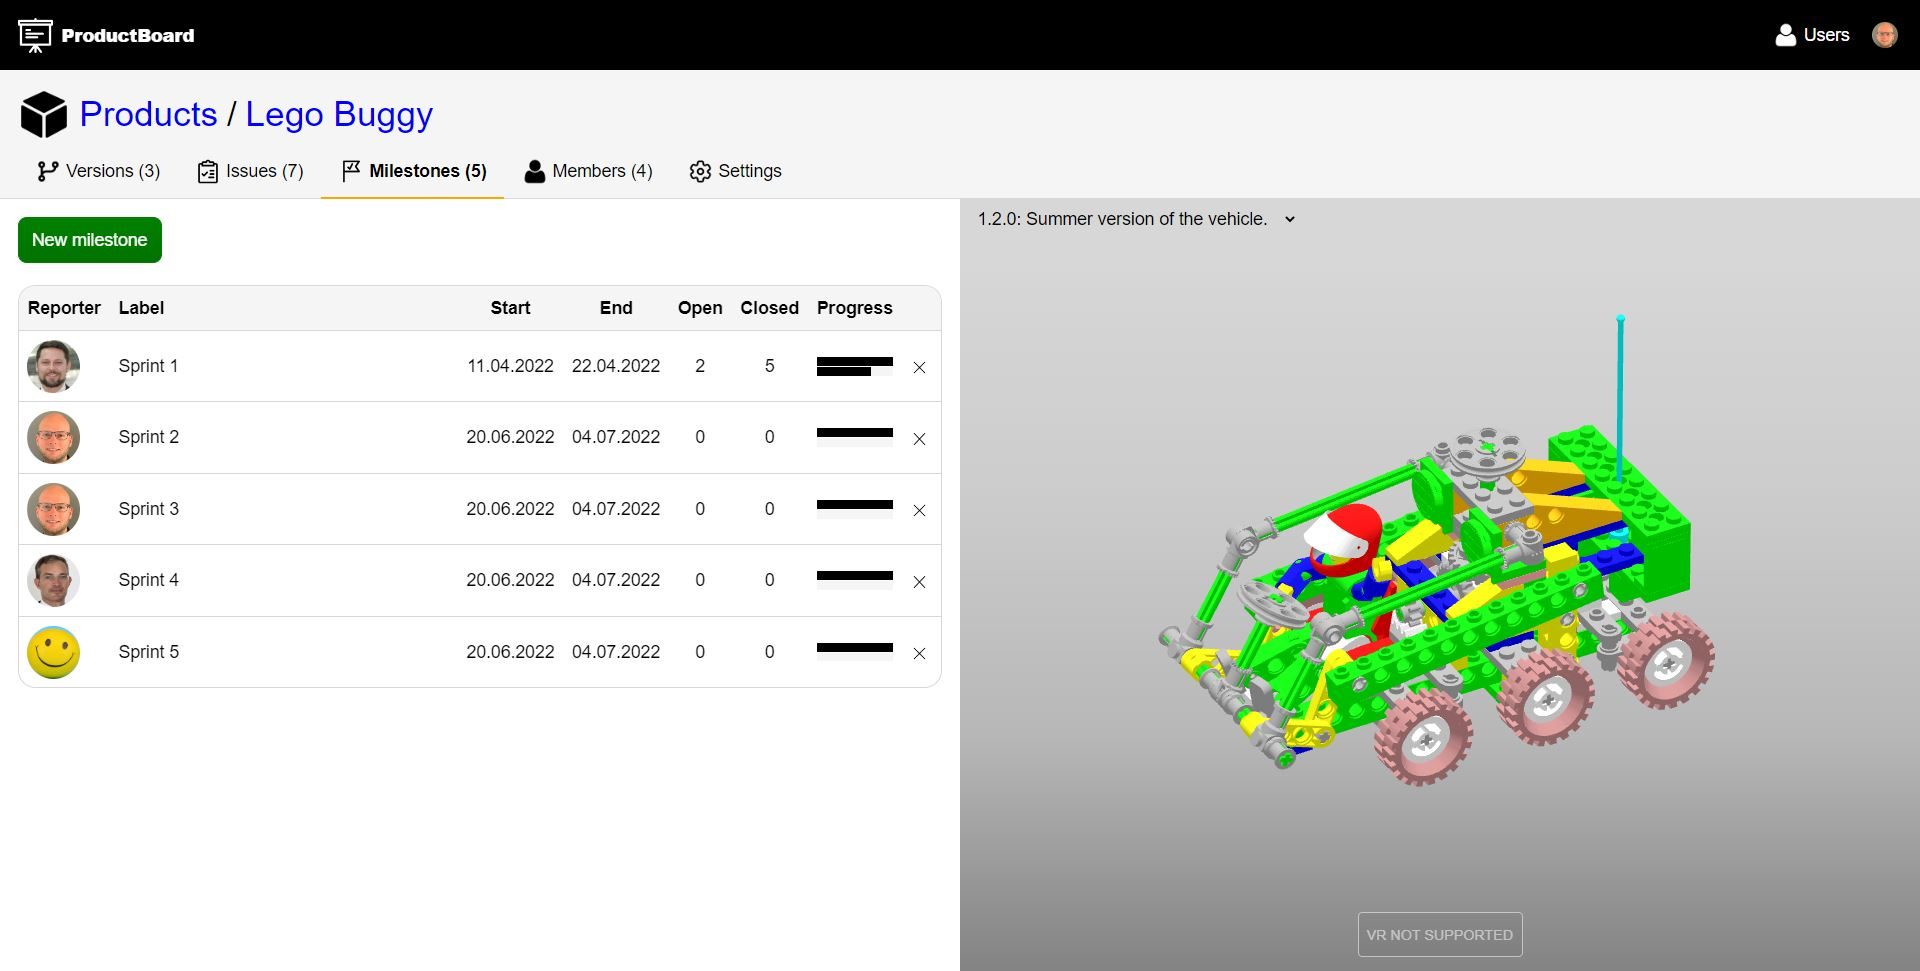
\includegraphics[width=7cm]{milestoneview.JPG}
        \caption{Milestone view}
        \label{fig: milestoneview}
    \end{figure}

    \begin{figure}[h]
        \centering
        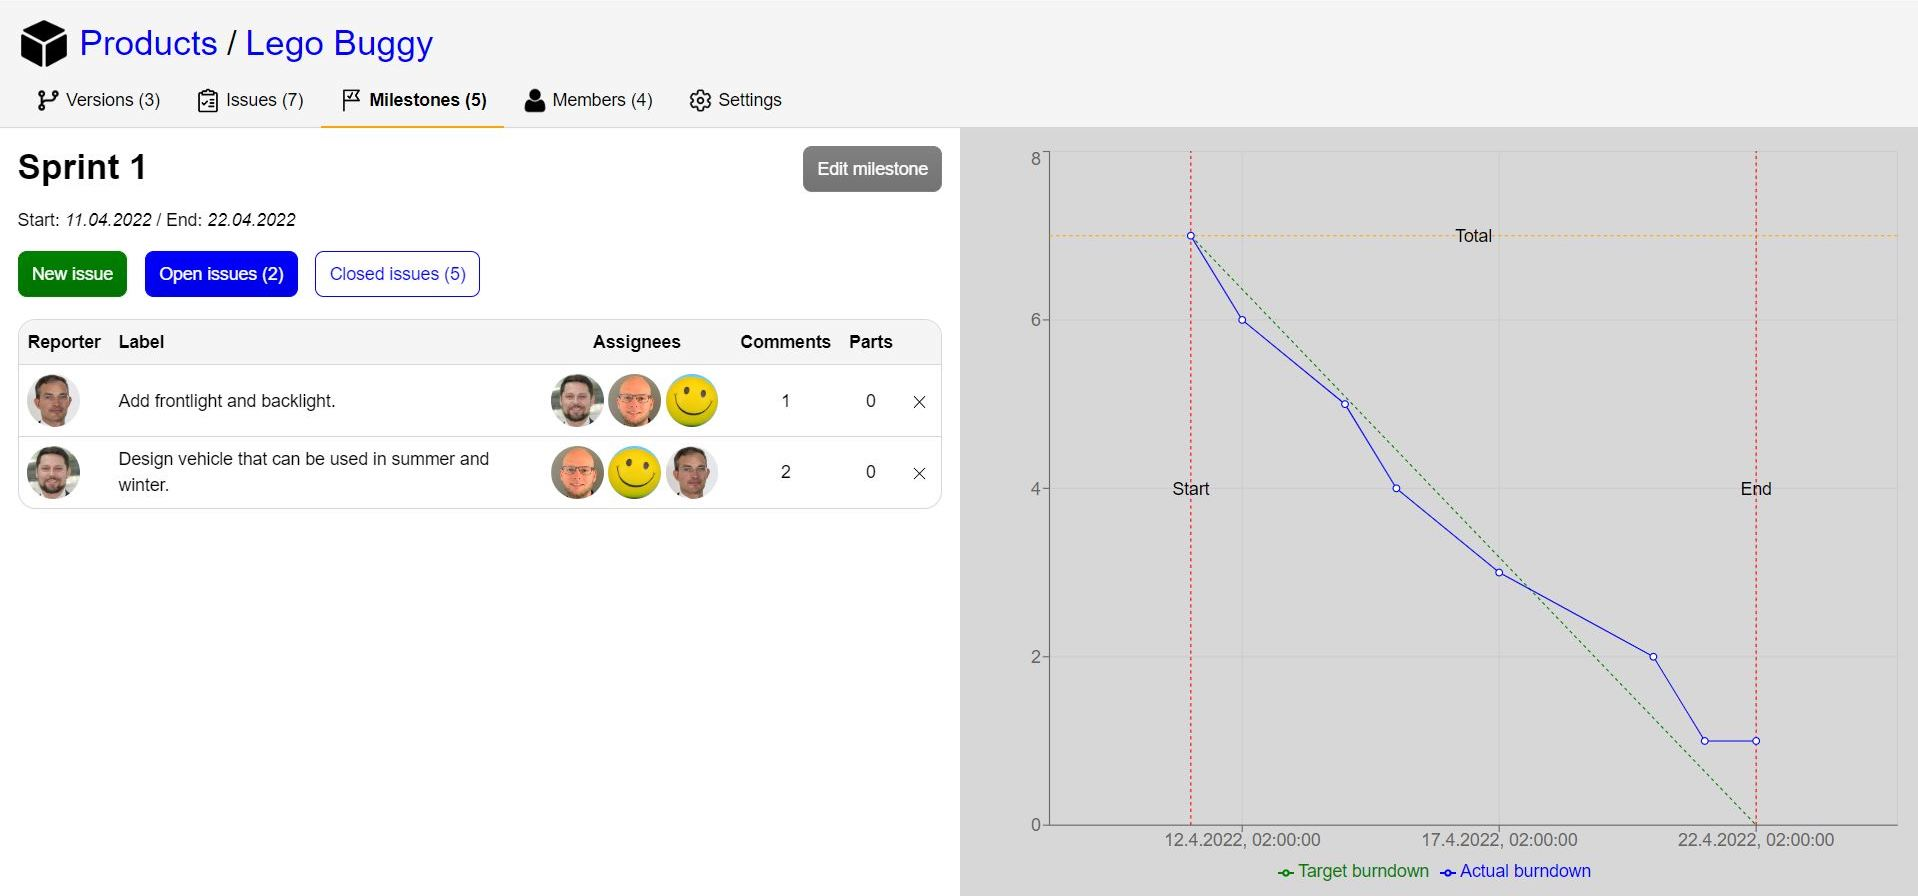
\includegraphics[width=7cm]{sprintview.JPG}
        \caption{Sprint view}
        \label{fig: sprintview}
    \end{figure}

    \begin{figure}[h]
        \centering
        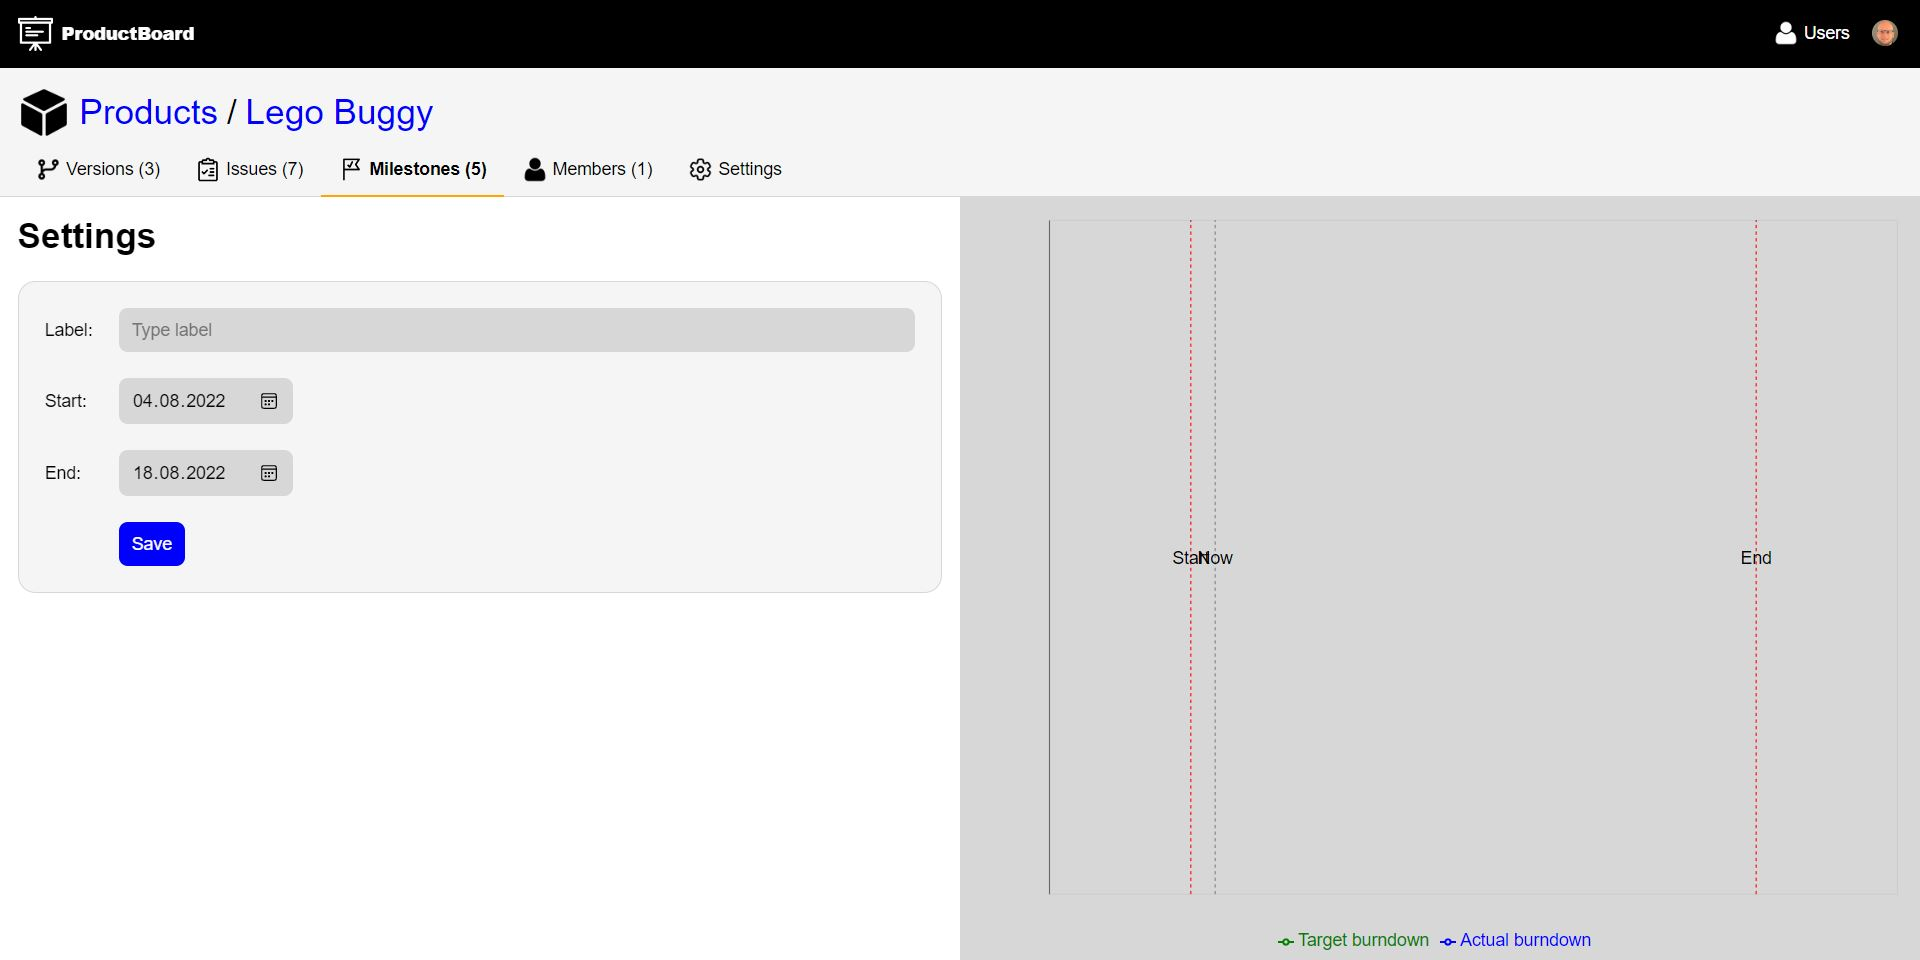
\includegraphics[width=7cm]{milestonesettingsview.JPG}
        \caption{Milestone Settings view}
        \label{fig: milestonesettingsview}
    \end{figure}

    \subsubsection*{Member view}
    To distribute the rights for a product, members are added to an existing product via the user interface. In the member view, a table shows all members who have access to the selected product [see Fig. \ref{fig: memberview} on page~\pageref{fig: memberview}]. The table shows the user picture and the name of the user. The column Role defines which rights the respective member has. At the moment there are three roles: manager, engineer, customer. As with every overview table, objects can be deleted from the list by clicking on the X button. The button New Member leads to the Member settings. Here you can enter the name of a potential member into a text field. When typing, a list appears in the lower area that filters for each new letter. If you click on a user from the list, this user is selected and a member role can be assigned to him [see Fig. \ref{fig: membersettingsview} on page~\pageref{fig: membersettingsview}]. If you click on X, the user disappears and the text field appears again. However, if Save is clicked, the current member is saved as specified and displayed in the member view.
    
    \begin{figure}[h]
        \centering
        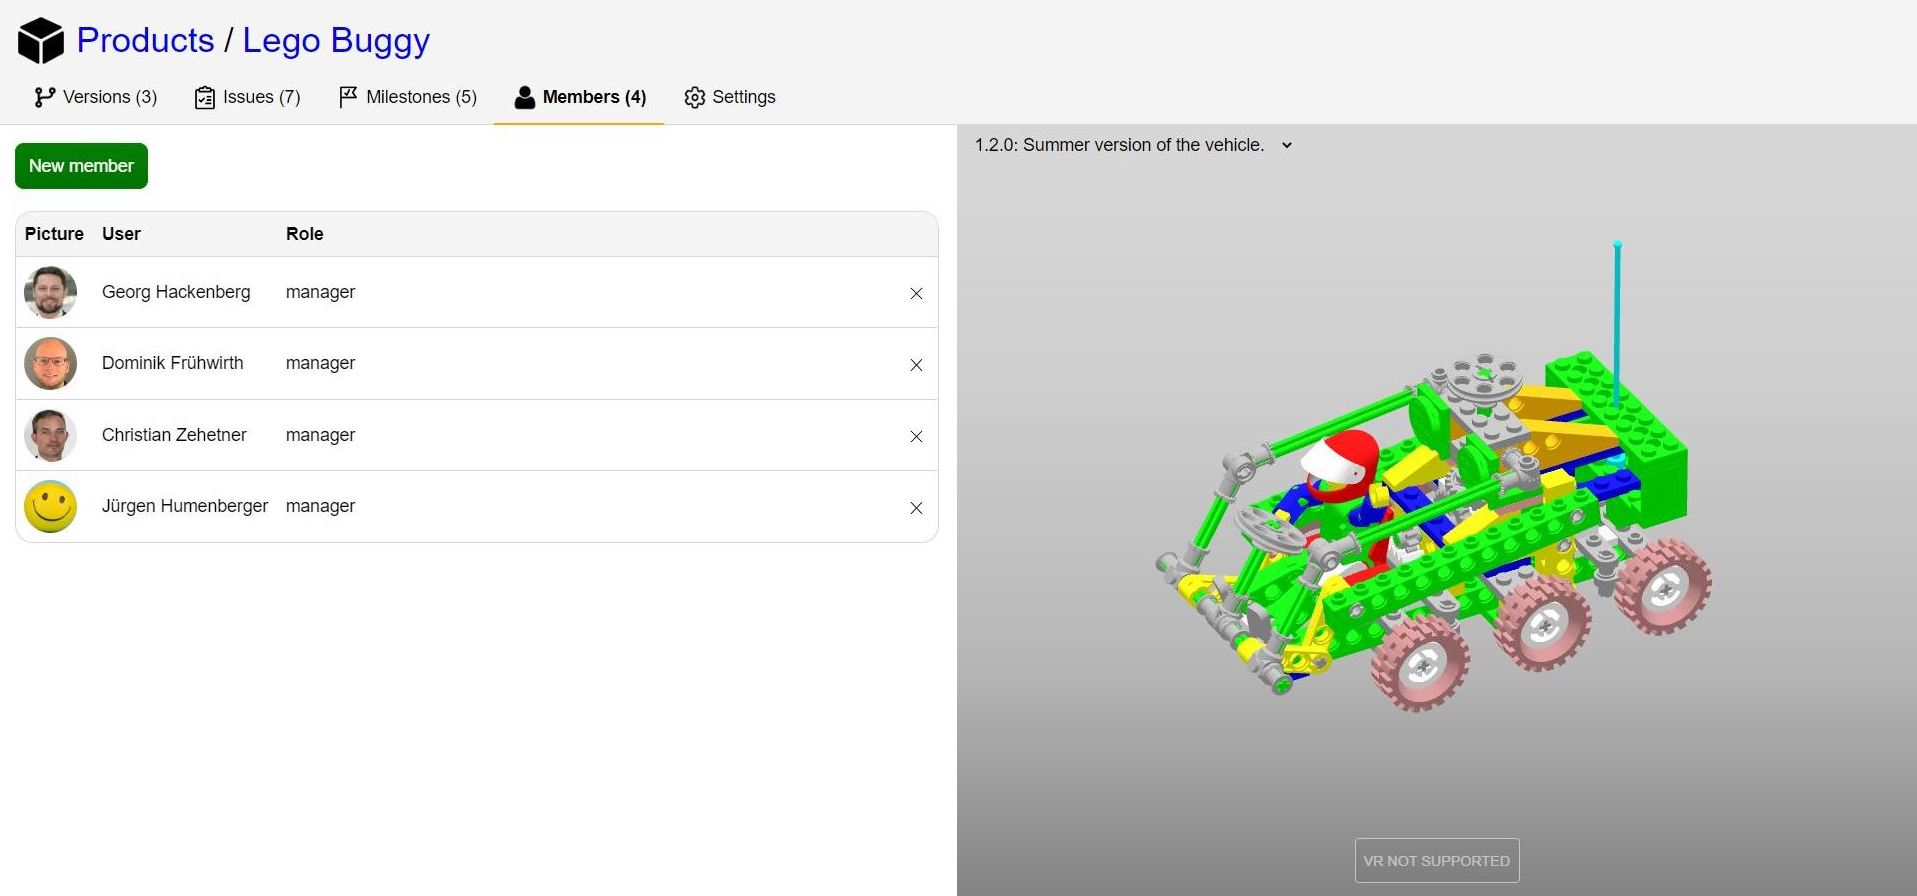
\includegraphics[width=7cm]{memberview.JPG}
        \caption{Member view}
        \label{fig: memberview}
    \end{figure}

    \begin{figure}[h]
        \centering
        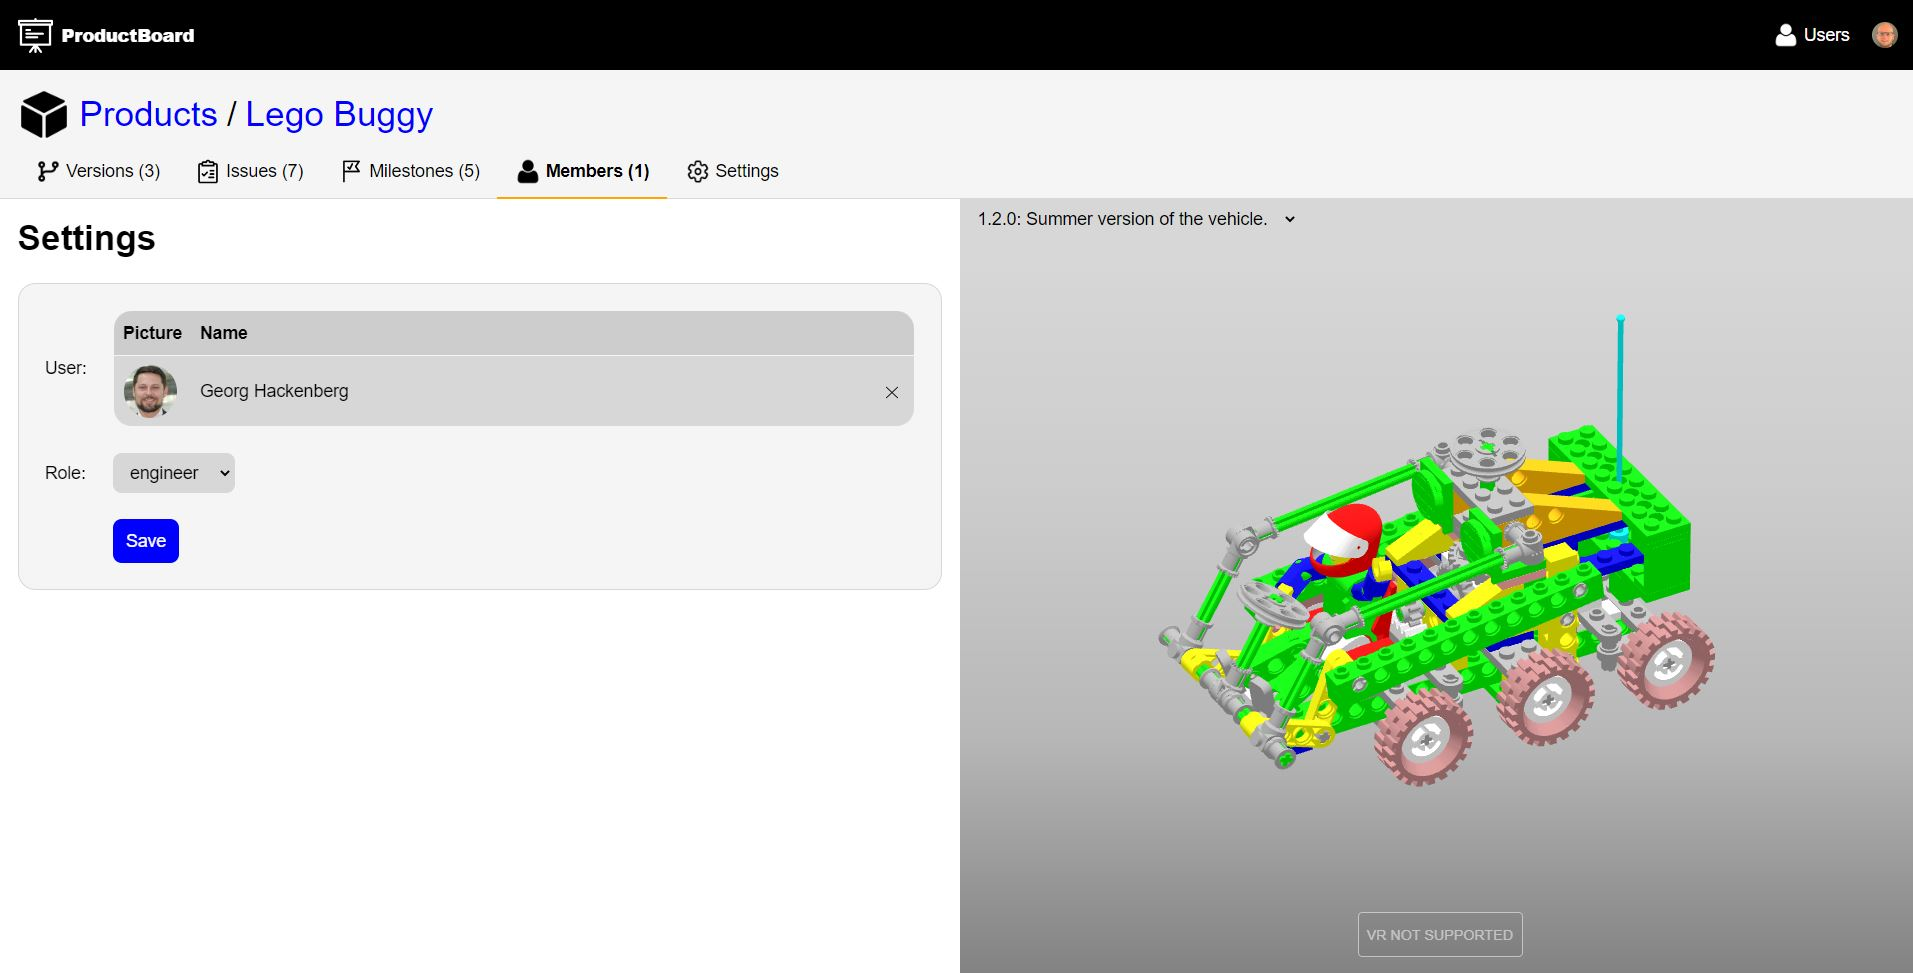
\includegraphics[width=7cm]{membersettingsview.JPG}
        \caption{Membersettings view}
        \label{fig: membersettingsview}
    \end{figure}

    \subsubsection*{Productsettings view}
    In this view the attributes Name and Description of the selected product can be changed [see Fig. \ref{fig: productsettingsview} on page~\pageref{fig: productsettingsview}]. After clicking the Save button the changes are visible in the product overview
    \begin{figure}[h]
        \centering
        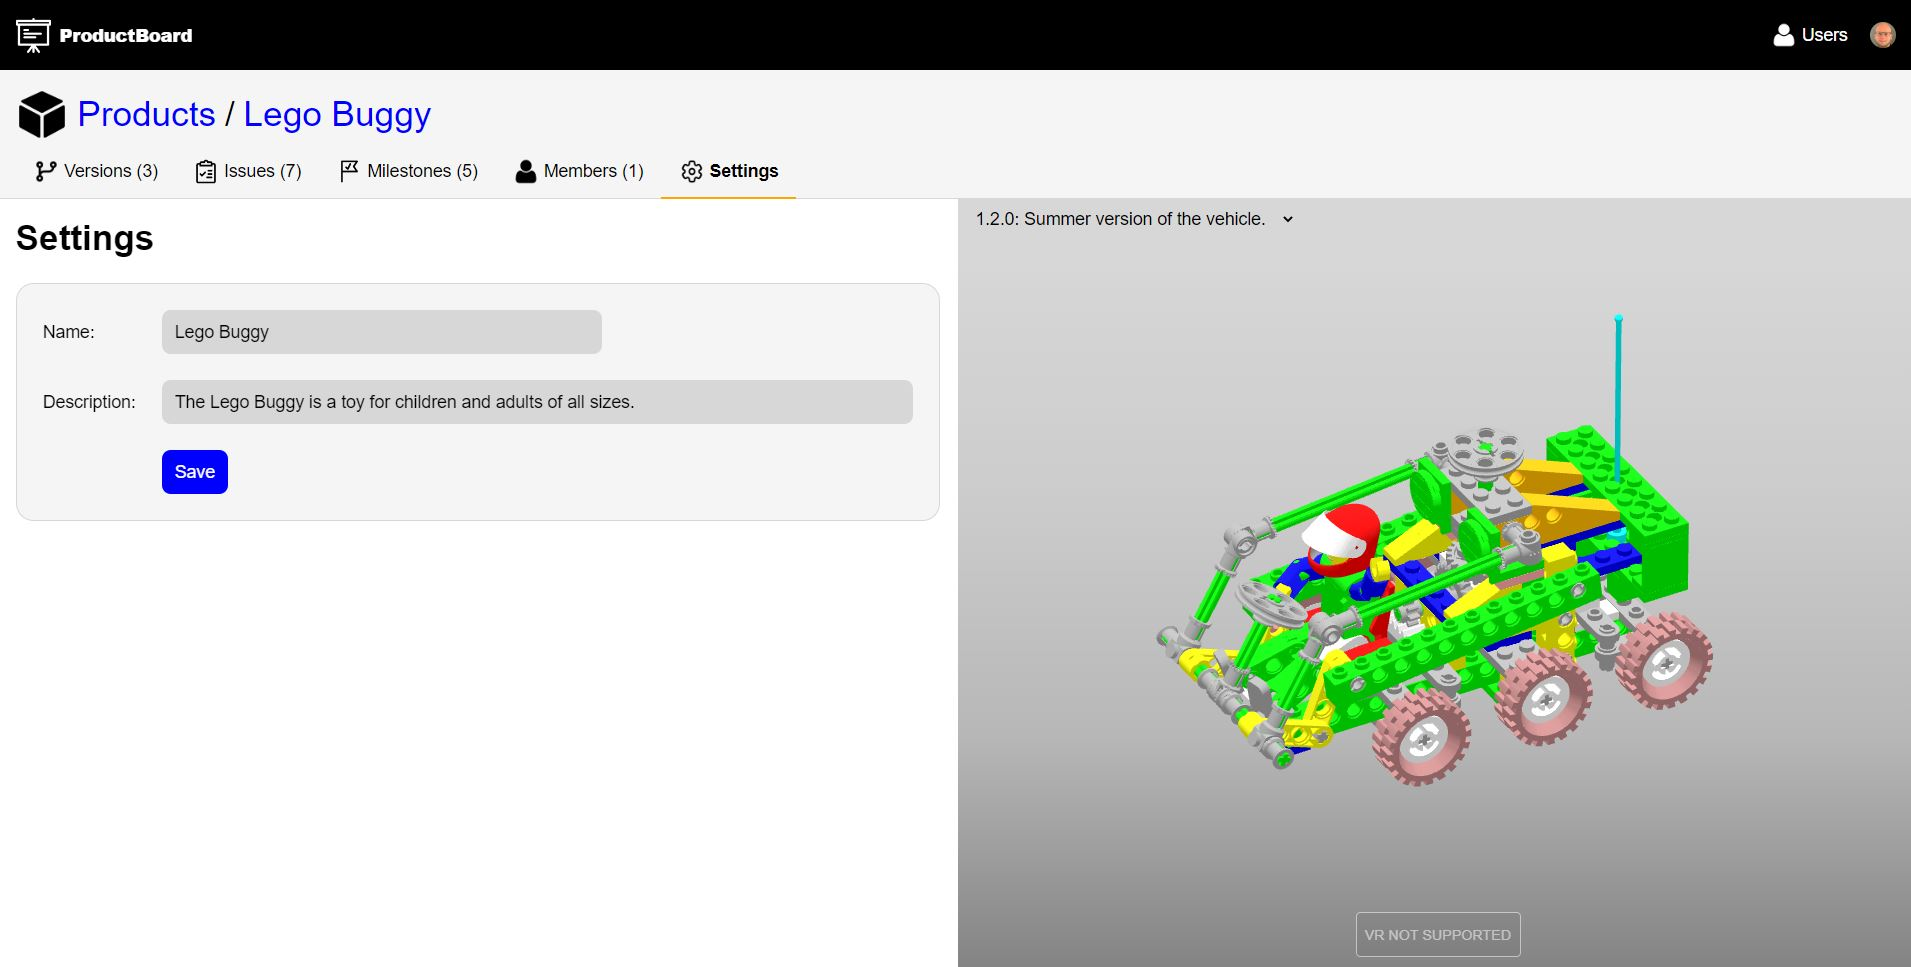
\includegraphics[width=7cm]{productsettingsview.JPG}
        \caption{Productsettings view}
        \label{fig: productsettingsview}
    \end{figure}